%======================================================================
% MODULE 2: Equation-Based Modelling and Hybrid Systems
%
% Learning Objectives:
% After completing this module, students will be able to:
% - Explain the advantages of acausal equation-based modelling
% - Build multi-domain models using Modelica or Simscape
% - Define and analyze hybrid systems with discrete modes and continuous dynamics
% - Identify and prevent Zeno behavior in hybrid models
% - Select appropriate numerical solvers for quadrotor simulation
% - Implement flight mode state machines in Stateflow
%======================================================================

\chapter{Equation-Based Modelling}
\index{equation-based modelling}

\section{Introduction: Why Equation-Based Modelling?}

In Module 1, we derived the equations of motion for a quadrotor: Newton's laws for translation, Euler's equations for rotation, and motor thrust models. These equations describe the physics. But how do we turn them into a working simulation?

This question is more subtle than it might appear. The equations we write on paper are \textbf{declarative}---they state relationships between quantities. But a computer simulation is \textbf{procedural}---it needs a sequence of instructions that compute outputs from inputs. Bridging this gap is the central challenge of simulation.

\subsection{The Traditional Approach: Block Diagrams}

The traditional approach is to manually rearrange equations into \emph{explicit} form:
\[
\dot{x} = f(x, u)
\]
and then implement this as a block diagram in Simulink, where each block computes one part of $f$.

\textbf{Why this is the traditional approach}: Block diagrams mirror the way we think about causality---inputs flow through blocks to produce outputs. This worked well for simple control systems where the signal flow is clear (e.g., reference $\to$ controller $\to$ plant $\to$ output).

\textbf{Problems with this approach}:
\begin{itemize}
    \item \textbf{Manual algebra}: You must solve for derivatives by hand, which is error-prone for complex systems. For a quadrotor with 12 states and 4 inputs, this involves substantial manipulation.
    \item \textbf{Fixed causality}: Once you decide that voltage is input and current is output, you cannot easily reverse this. But physics doesn't care about causality---Ohm's law $v = Ri$ relates $v$ and $i$ without specifying which is ``input.''
    \item \textbf{Poor reusability}: A motor model designed for one context may not work in another without re-derivation. If your motor model outputs torque from voltage, you cannot directly use it in a context where you need voltage from torque.
    \item \textbf{Multi-domain difficulty}: Connecting electrical, mechanical, and thermal subsystems requires careful manual bookkeeping of energy flow and conservation laws.
\end{itemize}

\subsection{The Equation-Based Approach}

\begin{keyidea}[title=The Core Idea]
Instead of telling the computer \emph{how} to compute (assignments), we tell it \emph{what} relationships hold (equations). The computer automatically determines how to solve them.

\textbf{Traditional (causal)}:
\begin{lstlisting}[language=C]
i = v / R;  // Current is computed FROM voltage
\end{lstlisting}

\textbf{Equation-based (acausal)}:
\begin{lstlisting}[language=Pascal]
R * i = v;  // Relationship holds; causality determined later
\end{lstlisting}
\end{keyidea}

\textbf{Why this matters for quadrotors}:
\begin{itemize}
    \item A motor model can be reused whether you're computing torque from voltage or back-EMF from speed.
    \item Connecting a battery, ESC, motor, and propeller ``just works''---the tool figures out the math.
    \item Physical constraints (conservation laws) are automatically enforced.
\end{itemize}

\section{Acausal Modelling}

\begin{definition}[Acausal Model]
\index{acausal model}
An \textbf{acausal model}\index{acausal model|textbf} describes a system using equations without specifying which variables are inputs and which are outputs. The causality is determined automatically when the model is compiled, based on how components are connected.
\end{definition}

\textbf{Why ``acausal''?} The term means ``without cause''---not in the philosophical sense, but in the computational sense. We don't specify what causes what; we only specify what relationships must hold. The compiler figures out the causal (computational) structure from the model topology.

\textbf{Intuition}: Think of physical components. A resistor doesn't ``know'' whether it's being driven by a voltage source or a current source. It simply obeys Ohm's law. Acausal modelling captures this physical reality directly.

\subsection{A Simple Example: The Resistor}

Consider Ohm's law for a resistor:
\[
v = R \cdot i
\]

In a \textbf{causal} (traditional) implementation, you must choose:
\begin{itemize}
    \item $i = v/R$ (voltage in, current out), OR
    \item $v = R \cdot i$ (current in, voltage out)
\end{itemize}

In an \textbf{acausal} implementation, you simply write the equation:
\begin{lstlisting}[language=Pascal]
R * i = v;
\end{lstlisting}

The tool determines causality based on what's connected. If this resistor is connected to a voltage source, current becomes the output. If connected to a current source, voltage becomes the output.

\begin{keyidea}[title=Reusability Through Acausality]
The same resistor model works in \emph{any} circuit, regardless of what it's connected to. This dramatically improves model reusability and reduces errors from manual re-derivation.
\end{keyidea}

\subsection{Intuition: Physical vs. Computational Thinking}

\textbf{Physical thinking}: ``A resistor obeys $v = Ri$. Period. It doesn't care which variable is 'input' or 'output'.''

\textbf{Computational thinking}: ``I need to compute something. What's given? What do I solve for?''

Acausal modelling lets you think physically while the computer handles the computational details.

\section{Languages and Tools}

Two major equation-based modelling ecosystems exist:

\subsection{Modelica}
\index{Modelica}

Modelica~\cite{fritzson2014principles} is an open, object-oriented modeling language for multi-domain physical systems.

\begin{itemize}
    \item \textbf{Open standard}: The language specification is freely available.
    \item \textbf{Multiple implementations}:
    \begin{itemize}
        \item Commercial: Dymola (Dassault), Wolfram SystemModeler
        \item Open-source: OpenModelica, JModelica
    \end{itemize}
    \item \textbf{Extensive libraries}: Modelica Standard Library includes electrical, mechanical, thermal, fluid domains.
    \item \textbf{Industry adoption}: Automotive (Ford, Toyota), aerospace (Airbus), energy systems.
\end{itemize}

\textbf{History}: Initiated in 1996 by Hilding Elmqvist (Lund, Sweden), building on ideas from his PhD thesis on structured modelling.

\subsection{Simscape (MATLAB/Simulink)}
\index{Simscape}

\begin{itemize}
    \item \textbf{Tight integration}: Works seamlessly with Simulink, Stateflow, and MATLAB.
    \item \textbf{Same concepts}: Acausal modelling, physical connections, automatic equation sorting.
    \item \textbf{Domain libraries}: Simscape Electrical, Simscape Multibody, Simscape Fluids.
    \item \textbf{Vendor lock-in}: Proprietary to MathWorks.
\end{itemize}

\begin{notebox}[title=Choosing Between Modelica and Simscape]
\textbf{Use Modelica} if:
\begin{itemize}
    \item You need an open, portable model format
    \item You're collaborating with partners using different tools
    \item You want access to community-developed libraries
\end{itemize}

\textbf{Use Simscape} if:
\begin{itemize}
    \item Your control design is in Simulink/MATLAB
    \item You need tight integration with code generation
    \item Your organization already uses the MathWorks toolchain
\end{itemize}

For this course, we use Simscape due to its integration with Simulink for control design.
\end{notebox}

\section{Modelica Language Fundamentals}

Even if using Simscape, understanding Modelica syntax helps read documentation and examples.

\subsection{Basic Structure}

\begin{lstlisting}[language=Pascal, caption=Basic Modelica class structure]
class ClassName "Description string"
  // Declarations
  Real x(start = 0) "State variable";
  parameter Real k = 1.0 "Constant parameter";

equation
  // Equations (not assignments!)
  der(x) = -k * x;  // der() is the derivative

end ClassName;
\end{lstlisting}

Key elements:
\begin{itemize}
    \item \texttt{Real}: Continuous variable type
    \item \texttt{parameter}: Constant during simulation (can be changed between runs)
    \item \texttt{start}: Initial condition
    \item \texttt{der(x)}: Time derivative $\dot{x}$
    \item \texttt{equation}: Section containing equations (not assignments)
\end{itemize}

\subsection{Example: Van der Pol Oscillator}

\begin{lstlisting}[language=Pascal, caption=Van der Pol oscillator---a nonlinear system]
class VanDerPol "Van der Pol oscillator model"
  Real x(start = 1) "First state";
  Real y(start = 1) "Second state";
  parameter Real lambda = 0.3 "Nonlinearity parameter";
equation
  der(x) = y;
  der(y) = -x + lambda*(1 - x*x)*y;
end VanDerPol;
\end{lstlisting}

\textbf{Interpretation}: This is a second-order nonlinear ODE. The \texttt{equation} section directly mirrors the mathematical formulation---no manual rearrangement needed.

\section{Connectors and Physical Connections}

The real power of acausal modelling comes from \emph{connectors}---interfaces that enforce physical laws automatically.

\textbf{Motivation}: When you connect two electrical components, Kirchhoff's laws must hold at the connection point. When you connect two mechanical elements, forces must balance. These are not arbitrary rules---they express conservation of energy and charge. A good modelling framework should enforce these automatically, not require the modeller to add them manually (which is error-prone).

\subsection{Connector Variables: Potential and Flow}

Physical systems exchange energy through pairs of conjugate variables. This classification comes from bond graph theory and energy-based modelling.

\begin{notebox}[title=Assumption: Lumped Parameter Systems]
The potential-flow classification assumes \textbf{lumped parameter} systems where energy storage and dissipation are localized. This is valid when the physical dimensions are small compared to the wavelength of signals. For a quadrotor motor running at 20,000 RPM with electrical dynamics under 10 kHz, this assumption holds well. It would not hold for radio-frequency circuits or long transmission lines.
\end{notebox}

\begin{center}
\begin{tabular}{llll}
\toprule
\textbf{Domain} & \textbf{Potential (Across)} & \textbf{Flow (Through)} & \textbf{Power} \\
\midrule
Electrical & Voltage $v$ & Current $i$ & $P = v \cdot i$ \\
Translational & Velocity $v$ & Force $F$ & $P = v \cdot F$ \\
Rotational & Angular velocity $\omega$ & Torque $\tau$ & $P = \omega \cdot \tau$ \\
Hydraulic & Pressure $p$ & Volume flow $\dot{V}$ & $P = p \cdot \dot{V}$ \\
Thermal & Temperature $T$ & Heat flow $\dot{Q}$ & $P = T \cdot \dot{Q}$ \\
\bottomrule
\end{tabular}
\end{center}

\begin{keyidea}[title=Connection Rules]
When connectors are joined:
\begin{itemize}
    \item \textbf{Potential variables} are set \textbf{equal} (same voltage, same velocity)
    \item \textbf{Flow variables} sum to \textbf{zero} (Kirchhoff's current law, force balance)
\end{itemize}
These rules automatically enforce conservation of energy.
\end{keyidea}

\subsection{Connector Definitions in Modelica}

\begin{lstlisting}[language=Pascal, caption=Electrical and mechanical connectors]
connector ElectricalPin
  Voltage v;        // Potential variable
  flow Current i;   // Flow variable (note 'flow' keyword)
end ElectricalPin;

connector MechanicalFlange
  Angle phi;        // Potential: angular position
  flow Torque tau;  // Flow: torque
end MechanicalFlange;
\end{lstlisting}

The \texttt{flow} keyword tells the compiler to use sum-to-zero equations for that variable.

\subsection{The Connect Equation}

\begin{lstlisting}[language=Pascal]
connect(component1.port, component2.port);
\end{lstlisting}

This generates:
\begin{itemize}
    \item Equality equations for potential variables: $v_1 = v_2$
    \item Sum-to-zero for flow variables: $i_1 + i_2 = 0$
\end{itemize}

\section{Multi-Domain Modelling: DC Motor Example}

A DC motor connects electrical and mechanical domains---current produces torque, and rotation produces back-EMF.

\begin{lstlisting}[language=Pascal, caption=DC motor model in Modelica]
model DCMotor
  // Components
  Resistor R(R = 0.5);           // Armature resistance
  Inductor L(L = 0.01);          // Armature inductance
  EMF emf(k = 0.1);              // Electromechanical coupling
  Inertia J(J = 0.001);          // Rotor inertia
  Damper b(d = 0.0001);          // Viscous friction
  Ground elecGnd;                // Electrical ground
  Fixed mechGnd;                 // Mechanical ground (fixed frame)

  // Connectors for external connection
  ElectricalPin p, n;            // Positive and negative terminals
  MechanicalFlange shaft;        // Output shaft

equation
  // Electrical connections
  connect(p, R.p);
  connect(R.n, L.p);
  connect(L.n, emf.p);
  connect(emf.n, n);
  connect(n, elecGnd.p);

  // Mechanical connections
  connect(emf.flange, J.flange_a);
  connect(J.flange_b, shaft);
  connect(J.flange_a, b.flange_a);
  connect(b.flange_b, mechGnd.flange);

end DCMotor;
\end{lstlisting}

\textbf{What the tool does automatically}:
\begin{enumerate}
    \item Collects all equations from components (Ohm's law, Faraday's law, Newton's second law)
    \item Generates connection equations (voltage equalities, current sums)
    \item Sorts equations into computable order
    \item Solves algebraic loops if needed
    \item Generates efficient simulation code
\end{enumerate}

\section{Application: Quadrotor Motor-Propeller System}

Let us apply equation-based modelling to the motor-propeller subsystem that converts PWM commands to thrust. This is a multi-domain system: electrical (motor windings), mechanical (rotor dynamics), and aerodynamic (propeller thrust and drag).

\textbf{Why model this in detail?} For basic simulation, a simple $T = b\omega^2$ model suffices. But understanding the full motor-propeller dynamics is essential for:
\begin{itemize}
    \item Predicting transient response (how fast can thrust change?)
    \item Designing motor controllers that improve response
    \item Understanding failure modes (motor saturation, thermal limits)
    \item Optimizing propeller-motor matching for efficiency
\end{itemize}

\subsection{System Overview}

\begin{center}
\begin{tabular}{ccccc}
PWM & $\rightarrow$ & ESC & $\rightarrow$ & Motor \\
(0-100\%) & & (voltage modulation) & & (electrical $\rightarrow$ mechanical) \\
\\
& & & & $\downarrow$ \\
\\
Thrust & $\leftarrow$ & Propeller & $\leftarrow$ & Shaft \\
(force + torque) & & (mechanical $\rightarrow$ aerodynamic) & & (torque, speed)
\end{tabular}
\end{center}

\subsection{Component Models}

\textbf{ESC (Electronic Speed Controller)}:
\begin{notebox}[title=Assumption: Ideal ESC]
We model the ESC as an ideal voltage source proportional to the PWM duty cycle:
\[
V_{motor} = \text{PWM} \cdot V_{battery}
\]
This ignores switching dynamics and ESC current limits. For most flight conditions, this is adequate.
\end{notebox}

\textbf{Brushless DC Motor}:
\begin{align}
L \frac{di}{dt} &= V - Ri - k_e \omega \quad \text{(electrical dynamics)} \\
J \frac{d\omega}{dt} &= k_t i - \tau_{load} - b\omega \quad \text{(mechanical dynamics)}
\end{align}

where:
\begin{itemize}
    \item $k_e$: Back-EMF constant [V/(rad/s)]
    \item $k_t$: Torque constant [Nm/A]
    \item For an ideal motor: $k_e = k_t$ (from energy conservation)
\end{itemize}

\begin{notebox}[title=Assumptions in the Motor Model]
\begin{enumerate}
    \item \textbf{Linear magnetics}: The motor operates in the linear region of its B-H curve (no saturation). This is valid for normal operating currents.
    \item \textbf{No cogging torque}: We ignore the position-dependent torque ripple from motor pole interactions. This is a good approximation for time-averaged behavior.
    \item \textbf{Averaged three-phase}: We model the three-phase motor as an equivalent single-phase DC motor, valid when the ESC commutation is much faster than mechanical dynamics.
    \item \textbf{Constant parameters}: $R$, $L$, $k_e$, $k_t$ are constant. In reality, $R$ increases with temperature (by $\sim$0.4\%/°C for copper).
\end{enumerate}
\end{notebox}

\textbf{Intuition}: The electrical equation is Kirchhoff's voltage law around the motor circuit: applied voltage equals resistive drop plus inductive voltage plus back-EMF (a voltage source proportional to speed). The mechanical equation is Newton's second law for rotation: inertia times angular acceleration equals motor torque minus load torque minus friction.

\begin{notebox}[title=Assumption: First-Order Motor Dynamics]
For small motors with low inductance, the electrical time constant $\tau_e = L/R$ is very small (sub-millisecond). We can often simplify to first-order dynamics:
\[
\tau_m \dot{\omega} + \omega = K \cdot \text{PWM}
\]
where $\tau_m$ is the mechanical time constant and $K$ is the steady-state gain.
\end{notebox}

\textbf{Propeller}:
\begin{align}
T &= C_T \rho D^4 \omega^2 \quad \text{(thrust)} \\
Q &= C_Q \rho D^5 \omega^2 \quad \text{(drag torque)}
\end{align}

This matches Module 1's $T = b\omega^2$ and $Q = k\omega^2$ with:
\[
b = C_T \rho D^4, \quad k = C_Q \rho D^5
\]

\begin{notebox}[title=Assumptions in the Propeller Model]
\begin{enumerate}
    \item \textbf{Hover or low-speed flight}: These equations assume the propeller operates in nearly static air. In forward flight, the advance ratio changes, and $C_T$, $C_Q$ become functions of the inflow.
    \item \textbf{No ground effect}: Near the ground (within about one rotor diameter), thrust increases significantly due to air being trapped between the propeller and ground.
    \item \textbf{Quasi-steady aerodynamics}: The propeller instantly produces thrust proportional to $\omega^2$. This is valid when aerodynamic time scales are much faster than mechanical time scales.
    \item \textbf{Constant air density}: We assume $\rho$ is constant at sea-level standard conditions. At altitude, lower $\rho$ reduces thrust for the same RPM.
\end{enumerate}
\end{notebox}

\textbf{Intuition}: Why $\omega^2$? Thrust is proportional to the momentum imparted to air. The momentum flow rate is (mass flow rate) $\times$ (exit velocity). Both increase linearly with $\omega$, giving $\omega^2$ dependence. The diameter appears as $D^4$ because thrust scales with disk area ($D^2$) and with the square of tip speed ($D^2$).

\subsection{Simscape Implementation}

This section provides a complete, working Simscape implementation of the motor-propeller system.

\subsubsection{Custom Propeller Component}

First, we create a custom Simscape component for the propeller aerodynamics. Save this as \texttt{Propeller.ssc}:

\begin{lstlisting}[language=Matlab, caption=Propeller.ssc - Custom Simscape propeller component]
component Propeller
% Propeller
% Converts rotational motion to thrust and drag torque
% using aerodynamic coefficients.
%
% Thrust: T = CT * rho * D^4 * omega^2
% Torque: Q = CQ * rho * D^5 * omega^2

nodes
    R = foundation.mechanical.rotational.rotational;  % Shaft:right
end

outputs
    T = {0, 'N'};         % Thrust:right
end

parameters
    CT = {0.1, '1'};           % Thrust coefficient
    CQ = {0.01, '1'};          % Torque coefficient
    D = {0.1, 'm'};            % Propeller diameter
    rho = {1.225, 'kg/m^3'};   % Air density
    direction = {1, '1'};      % Rotation direction (+1 or -1)
end

variables
    w = {0, 'rad/s'};          % Angular velocity
    tau = {0, 'N*m'};          % Reaction torque
end

branches
    tau : R.t -> *;            % Torque flows into the shaft
end

equations
    w == R.w;                                          % Get angular velocity
    T == direction * CT * rho * D^4 * w * abs(w);     % Thrust (signed)
    tau == CQ * rho * D^5 * w * abs(w);               % Drag torque
end
end
\end{lstlisting}

\subsubsection{ESC Component}

The Electronic Speed Controller converts PWM commands to motor voltage:

\begin{lstlisting}[language=Matlab, caption=ESC.ssc - Electronic Speed Controller]
component ESC
% Electronic Speed Controller
% Converts PWM command (0-1) to voltage output

nodes
    p = foundation.electrical.electrical;    % +:right
    n = foundation.electrical.electrical;    % -:right
end

inputs
    pwm = {0, '1'};                          % PWM command (0-1)
end

parameters
    V_batt = {3.7, 'V'};                     % Battery voltage
end

variables
    v = {0, 'V'};                            % Output voltage
    i = {0, 'A'};                            % Current
end

branches
    i : p.i -> n.i;
end

equations
    v == p.v - n.v;
    v == pwm * V_batt;
end
end
\end{lstlisting}

\subsubsection{Complete Motor-Propeller Subsystem}

Now we assemble the complete system in a Simscape model. The following MATLAB script creates the model programmatically:

See Listing~\ref{lst:simscape-model} (Appendix~\ref{app:code-listings}) for a complete MATLAB script that programmatically creates the motor-propeller Simscape model, including DC motor, propeller, sensors, and all connections.

\subsubsection{Testing the Motor-Propeller Model}

See Listing~\ref{lst:simscape-test} (Appendix~\ref{app:code-listings}) for a MATLAB test script that validates the motor-propeller model by applying a step input and analyzing the step response.

\subsubsection{Parameter Tuning to Match Hardware}

To match the Simscape model to actual Crazyflie motors:

See Listing~\ref{lst:simscape-param-id} (Appendix~\ref{app:code-listings}) for a MATLAB script that back-calculates motor parameters ($K_e$, $J$, $C_T$) from measured step response data.

\begin{keyidea}[title=Simscape Model Benefits]
The Simscape motor-propeller model automatically handles:
\begin{itemize}
    \item \textbf{Bidirectional coupling}: Propeller load affects motor speed
    \item \textbf{Transient dynamics}: Electrical and mechanical time constants
    \item \textbf{Energy conservation}: Power flow is consistent across domains
    \item \textbf{Parameterization}: Easy to adjust for different motors/propellers
\end{itemize}

This model can be connected to the quadrotor rigid-body dynamics for complete system simulation.
\end{keyidea}

\subsection{Ground Effect Modeling}
\index{ground effect}

When a quadrotor hovers close to the ground, the propeller thrust increases beyond what the standard thrust equation predicts. This phenomenon, called \textbf{ground effect}\index{ground effect|textbf}, significantly impacts low-altitude flight and landing.

\subsubsection{Physical Explanation}

Ground effect occurs because the ground surface restricts the downward flow of air from the propellers:

\begin{itemize}
    \item Air cannot accelerate downward indefinitely---the ground redirects it
    \item Higher pressure builds up beneath the propeller
    \item The propeller effectively operates at a higher induced velocity
    \item For the same power input, more thrust is generated
\end{itemize}

%----------------------------------------------------------------------
% FIGURE: Ground Effect Flow Visualization
%----------------------------------------------------------------------
% Description: Side-by-side comparison of propeller flow patterns.
%
% Left panel: "Free air" - Propeller with streamlines showing
%   downward flow accelerating away, vortex ring at tip.
%
% Right panel: "Ground effect" - Same propeller close to ground,
%   streamlines curving outward along ground surface, higher
%   pressure region indicated beneath propeller.
%
% Show height 'z' and propeller diameter 'D' for scale.
% Dimensions: Full width, ~5cm height.
%----------------------------------------------------------------------

\subsubsection{Ground Effect Model}

The standard thrust model gives:
\[
T_\infty = C_T \rho D^4 \omega^2
\]
where $T_\infty$ is the thrust in free air (far from the ground).

Near the ground, thrust is amplified by a factor that depends on the height-to-diameter ratio:
\[
T_{\text{ground}} = T_\infty \cdot \sigma(z/D)
\]

Several empirical models exist for $\sigma(z/D)$. A commonly used model based on blade element momentum theory is:

\begin{equation}
\sigma(z/D) = \frac{1}{1 - \left(\frac{R}{4z}\right)^2} \approx \frac{1}{1 - \left(\frac{D}{8z}\right)^2}
\label{eq:ground_effect}
\end{equation}

where $R = D/2$ is the propeller radius and $z$ is the height above ground.

\begin{example}[Ground Effect Magnitude]
For a quadrotor with 46 mm propellers ($D = 0.046$ m) at various heights:

\begin{center}
\begin{tabular}{ccc}
\toprule
Height $z$ (cm) & $z/D$ & Thrust Multiplier $\sigma$ \\
\midrule
2.3 (0.5D) & 0.5 & 1.066 \\
4.6 (1D) & 1.0 & 1.016 \\
9.2 (2D) & 2.0 & 1.004 \\
23 (5D) & 5.0 & 1.0006 \\
\bottomrule
\end{tabular}
\end{center}

At one diameter above ground, thrust is about 1.6\% higher than in free air. Ground effect becomes negligible above $z > 3D$.
\end{example}

\subsubsection{Alternative Ground Effect Models}

Several alternative formulations are used in the literature:

\textbf{Cheeseman-Bennett Model} (classic helicopter theory):
\[
\sigma(z/R) = \frac{1}{1 - (R/4z)^2}
\]

\textbf{Hayden Model} (better for small $z$):
\[
\sigma(z/R) = 1 + \frac{R^2}{8z^2} - \frac{R^4}{128z^4}
\]

\textbf{Sanchez-Cuevas et al.} (fitted for quadrotors):
\[
\sigma(z/R) = 1 + A \exp(-B \cdot z/R)
\]
with typical values $A \approx 0.4$ and $B \approx 3$.

\begin{notebox}[title=Model Selection]
The exponential model is often preferred for quadrotors because:
\begin{itemize}
    \item It smoothly approaches 1 as $z \to \infty$
    \item Parameters can be fitted to experimental data
    \item No singularity at $z = D/8$ (unlike the classical model)
\end{itemize}
\end{notebox}

\subsubsection{Implementation in Simulation}

Adding ground effect to our Simscape propeller model:

See Listing~\ref{lst:propeller-ge} (Appendix~\ref{app:code-listings}) for the complete Simscape component that implements the exponential ground effect model.

\subsubsection{Impact on Control}

Ground effect has several implications for flight control:

\begin{itemize}
    \item \textbf{Landing}: The quadrotor requires less throttle near the ground. If the controller doesn't account for this, it may descend faster than expected and bounce.

    \item \textbf{Takeoff}: Thrust appears to decrease as the quadrotor climbs out of ground effect, which can feel like the motors are losing power.

    \item \textbf{Low-altitude hover}: Without compensation, position control will have a steady-state error dependent on height.
\end{itemize}

\textbf{Feedforward Compensation}:

See Listing~\ref{lst:ground-effect-ctrl} (Appendix~\ref{app:code-listings}) for a C implementation of ground effect feedforward compensation in the altitude control loop.

\begin{warningbox}[title=Height Measurement Requirements]
Ground effect compensation requires accurate height-above-ground measurement. GPS altitude is not suitable because:
\begin{itemize}
    \item GPS accuracy is typically 2--5 m (ground effect occurs within 10 cm)
    \item GPS measures altitude above sea level, not above ground
\end{itemize}
Use a downward-facing range sensor (ultrasonic, infrared, or LiDAR) for ground effect compensation.
\end{warningbox}

\subsubsection{Experimental Identification}

To characterize ground effect for a specific quadrotor:

See Listing~\ref{lst:ground-effect-id} (Appendix~\ref{app:code-listings}) for a MATLAB script that identifies ground effect parameters from experimental thrust measurements at various heights.

\begin{keyidea}[title=When Ground Effect Matters]
Include ground effect in your simulation if:
\begin{itemize}
    \item Testing landing/takeoff control algorithms
    \item Operating primarily at low altitudes (indoor, warehouse)
    \item Requiring high position accuracy near the ground
    \item Validating simulation against real flight data
\end{itemize}

For general flight testing above 1 meter, ground effect can usually be neglected.
\end{keyidea}

\section{Model Translation Process}

Understanding how equation-based models become simulations:

\begin{enumerate}
    \item \textbf{Flattening}: Expand all component hierarchies into one large set of equations
    \item \textbf{Equation analysis}: Identify variables, equations, and their dependencies
    \item \textbf{Index reduction}: Handle higher-index DAEs (constraints that require differentiation)
    \item \textbf{Causality assignment}: Determine which variable is solved from which equation
    \item \textbf{Sorting}: Order equations so each uses only previously computed values
    \item \textbf{Algebraic loop handling}: Solve simultaneous equations where needed
    \item \textbf{Code generation}: Produce efficient C code for simulation
\end{enumerate}

\begin{notebox}[title=What Can Go Wrong]
\begin{itemize}
    \item \textbf{Structurally singular}: More unknowns than equations (under-constrained)
    \item \textbf{Over-constrained}: More equations than unknowns (contradictory constraints)
    \item \textbf{High-index DAE}: Constraints require repeated differentiation (numerical difficulties)
\end{itemize}
The tool will report these errors during compilation.
\end{notebox}

\section{Chapter Summary}

Equation-based modelling with Modelica or Simscape offers significant advantages for quadrotor development:

\begin{itemize}
    \item \textbf{Physical fidelity}: Write equations as they appear in textbooks
    \item \textbf{Reusability}: Same motor model works in any context
    \item \textbf{Multi-domain}: Naturally connects electrical, mechanical, and aerodynamic subsystems
    \item \textbf{Automatic solving}: No manual causality derivation
    \item \textbf{Error checking}: Tool catches missing equations or constraints
\end{itemize}

The tradeoff is less direct control over the solution process and a steeper learning curve for the tools.


\chapter{Hybrid Systems}
\index{hybrid system}

\section{Introduction: Why Hybrid Systems?}

So far, we have modelled systems with continuous dynamics: differential equations that evolve smoothly in time. But real quadrotor systems\index{hybrid system|textbf} have \emph{discrete} aspects too:

\begin{itemize}
    \item \textbf{Flight modes}: The controller switches between Idle, Armed, Hover, Position Control, Land
    \item \textbf{Sensor modes}: GPS available vs. GPS denied triggers different estimation algorithms
    \item \textbf{Failsafes}: Low battery triggers Return-to-Home; signal loss triggers Land
    \item \textbf{Physical events}: Landing gear contact, propeller stall, motor saturation
\end{itemize}

\textbf{Why study hybrid systems formally?} One might think: ``I'll just add some if-statements to my simulation.'' This works for simple cases but leads to problems:
\begin{itemize}
    \item \textbf{Numerical issues}: Standard ODE solvers assume smooth dynamics. Sudden changes can cause solver failures or inaccurate results.
    \item \textbf{Analysis difficulty}: How do you prove stability when the controller switches between different modes? Standard Lyapunov theory doesn't directly apply.
    \item \textbf{Subtle bugs}: What happens if two mode transitions are triggered simultaneously? The informal approach doesn't answer this.
    \item \textbf{Zeno behavior}: Under certain conditions, infinitely many mode switches occur in finite time---a pathological situation that stops simulation.
\end{itemize}

A formal hybrid systems framework addresses these issues systematically. The theory of hybrid automata was developed by Henzinger~\cite{henzinger1996theory} and provides a rigorous foundation for modeling and analyzing such systems. For a comprehensive treatment, see Goebel et al.~\cite{goebel2012hybrid}.

\begin{keyidea}[title=The Hybrid Nature of Quadrotors]
A quadrotor is inherently a \textbf{hybrid system}:
\begin{itemize}
    \item \textbf{Continuous dynamics}: Position, velocity, orientation evolve according to ODEs
    \item \textbf{Discrete modes}: Flight controller state machine switches between behaviors
    \item \textbf{Mode-dependent dynamics}: Different control laws apply in different modes
    \item \textbf{Discrete events}: Takeoff, landing, failsafe activation
\end{itemize}
Understanding hybrid systems is essential for designing robust flight software.
\end{keyidea}

\section{Formal Definition of Hybrid Systems}
\label{sec:hybrid-automaton-def}

\begin{definition}[Hybrid Automaton]
\index{hybrid automaton}
A \textbf{hybrid automaton}\index{hybrid automaton|textbf} $H$ is defined by the tuple:
\[
H = (Q, X, f, \text{Init}, D, E, G, R)
\]
where:
\begin{itemize}
    \item $Q$: Finite set of \textbf{discrete modes}
    \item $X \subseteq \mathbb{R}^n$: \textbf{Continuous state space}
    \item $f: Q \times X \rightarrow \mathbb{R}^n$: \textbf{Vector field} (dynamics in each mode)
    \item $\text{Init} \subseteq Q \times X$: \textbf{Initial states}
    \item $D: Q \rightarrow 2^X$: \textbf{Domain} (invariant) for each mode
    \item $E \subseteq Q \times Q$: \textbf{Edges} (allowed mode transitions)
    \item $G: E \rightarrow 2^X$: \textbf{Guard conditions} (when transitions may occur)
    \item $R: E \times X \rightarrow 2^X$: \textbf{Reset map} (how continuous state changes at transitions)
\end{itemize}
\end{definition}

\textbf{Semantics}: The system evolves continuously in mode $q$ according to $\dot{x} = f(q, x)$ while $x \in D(q)$. When $x \in G(e)$ for some edge $e = (q, q')$, a discrete transition \emph{may} occur, with the new state satisfying $x^+ \in R(e, x^-)$. If $x$ reaches the boundary of $D(q)$ and no guard is enabled, the system blocks (this indicates a modeling error).

\textbf{Understanding each component}:
\begin{itemize}
    \item \textbf{Modes $Q$}: Operating regimes with distinct dynamics. A quadrotor has modes like Hover, Land, Emergency.

    \item \textbf{Continuous state $X$}: Physical variables evolving according to ODEs---position, velocity, orientation.

    \item \textbf{Vector field $f$}: Mode-dependent dynamics. In Hover mode, thrust compensates gravity; in Emergency mode, thrust is reduced.

    \item \textbf{Domain $D$}: The region where continuous evolution is valid in each mode. The system \emph{must} leave mode $q$ before $x$ exits $D(q)$.

    \item \textbf{Guards $G$}: Conditions that \emph{enable} a transition. A transition may occur when $x \in G(e)$, but is not forced until $x$ exits the domain.

    \item \textbf{Reset map $R$}: How continuous state changes at a transition. Often $R(e, x) = \{x\}$ (no reset), but integrator states may be zeroed.
\end{itemize}

\begin{keyidea}[title=Domain vs. Guard]
The distinction between domain and guard is crucial:
\begin{itemize}
    \item \textbf{Domain $D(q)$}: Where the system \emph{can} stay in mode $q$. Leaving the domain \emph{forces} a transition.
    \item \textbf{Guard $G(e)$}: Where a transition \emph{may} occur. The transition is optional while inside the domain.
\end{itemize}
Example: In Landing mode, the domain might be $D(\text{Landing}) = \{x : z \geq -0.5\}$ (above 0.5m). The guard to Settled might be $G(\text{Landing} \to \text{Settled}) = \{x : z > -0.05 \land |v_z| < 0.1\}$. The quadrotor can transition to Settled when near the ground and slow, but \emph{must} transition (or to another mode) before exceeding the domain boundary.
\end{keyidea}

\section{Example: Quadrotor Landing Sequence}
\label{sec:landing-hybrid}

Rather than the classical bouncing ball example, we develop a hybrid automaton for the \textbf{quadrotor landing sequence}---a practically relevant scenario that connects to the dynamics and control material throughout this book.

\subsection{Physical Description}

Landing a quadrotor involves several distinct phases with different dynamics:
\begin{enumerate}
    \item \textbf{Descent}: The quadrotor descends at a controlled rate toward the landing zone
    \item \textbf{Ground effect}: As altitude decreases below approximately one rotor diameter, aerodynamic ground effect increases lift
    \item \textbf{Touchdown}: The landing gear contacts the ground, introducing contact forces
    \item \textbf{Settled}: Motors spin down and the quadrotor rests on the ground
\end{enumerate}

Each phase has fundamentally different dynamics, making this a natural hybrid system.

\subsection{Hybrid Automaton Formulation}

We define the landing hybrid automaton with continuous state $x = [z, \dot{z}, I_z]^T$ where $z$ is altitude (NED, so $z < 0$ means above ground), $\dot{z}$ is vertical velocity, and $I_z$ is the altitude controller integrator state.

Following the formal definition from Section~\ref{sec:hybrid-automaton-def}, we specify:

\begin{itemize}
    \item $Q = \{\text{Descent}, \text{GroundEffect}, \text{Contact}, \text{Settled}\}$
    \item $X = \mathbb{R}^3$ (altitude, velocity, integrator state)
    \item $\text{Init} = \{(\text{Descent}, x) : z < -h_{ge}, \dot{z} = 0\}$ (start above ground effect region)
\end{itemize}

\textbf{Vector fields} (simplified to vertical dynamics):

\textbf{Descent mode}:
\[
f_{\text{Descent}}(x) = \begin{bmatrix} \dot{z} \\ g - \frac{T}{m} \\ z_{target} - z \end{bmatrix}
\quad \text{where} \quad T = mg + K_p(z_{target} - z) + K_d(\dot{z}_{target} - \dot{z}) + K_i I_z
\]

\textbf{GroundEffect mode} (thrust augmented by ground effect factor $\sigma(z)$):
\[
f_{\text{GE}}(x) = \begin{bmatrix} \dot{z} \\ g - \frac{T \cdot \sigma(z)}{m} \\ z_{target} - z \end{bmatrix}
\quad \text{where} \quad \sigma(z) = \frac{1}{1 - (r/4z)^2}
\]
Here $r$ is the rotor radius and $z$ is height above ground (recall from Chapter~\ref{ch:quadrotor-dynamics} that $\sigma > 1$ near the ground).

\textbf{Contact mode} (spring-damper ground interaction):
\[
f_{\text{Contact}}(x) = \begin{bmatrix} \dot{z} \\ g - \frac{T}{m} + \frac{1}{m}(k_g z - c_g \dot{z}) \\ 0 \end{bmatrix}
\]
where $k_g$ and $c_g$ are ground stiffness and damping. Note the integrator is frozen.

\textbf{Settled mode}:
\[
f_{\text{Settled}}(x) = \begin{bmatrix} 0 \\ 0 \\ 0 \end{bmatrix}
\]

\textbf{Domains} (invariants for each mode):
\begin{align*}
D(\text{Descent}) &= \{x \in X : z \leq -h_{ge}\} \\
D(\text{GroundEffect}) &= \{x \in X : -h_{ge} < z < \delta\} \\
D(\text{Contact}) &= \{x \in X : z \geq -\delta\} \\
D(\text{Settled}) &= X \quad \text{(terminal mode)}
\end{align*}
The domain specifies where the system \emph{must} remain while in each mode. When the state reaches the boundary of the domain, a transition \emph{must} occur (if a guard is enabled) or the model is ill-posed.

\textbf{Edge set}:
\[
E = \{(\text{Descent}, \text{GroundEffect}), (\text{GroundEffect}, \text{Contact}), (\text{Contact}, \text{Settled}), (\text{Contact}, \text{GroundEffect})\}
\]

\textbf{Guard conditions}:
\begin{center}
\begin{tabular}{lll}
\toprule
\textbf{Transition} & \textbf{Guard $G$} & \textbf{Physical meaning} \\
\midrule
Descent $\to$ GroundEffect & $z > -h_{ge}$ & Altitude below ground effect threshold \\
GroundEffect $\to$ Contact & $z \geq 0$ & Landing gear touches ground \\
Contact $\to$ Settled & $|z| < \epsilon \land |\dot{z}| < v_{thresh}$ & Motion stopped \\
Contact $\to$ GroundEffect & $z < -\delta$ & Bounced back up \\
\bottomrule
\end{tabular}
\end{center}
where $h_{ge} \approx 2r$ is the ground effect onset altitude (typically 0.1--0.3 m for small quadrotors).

\textbf{Reset maps}:
\begin{itemize}
    \item Descent $\to$ GroundEffect: $R(x) = x$ (no reset, continuous transition)
    \item GroundEffect $\to$ Contact: $R(x) = [0, \dot{z}, 0]^T$ (clamp altitude, reset integrator)
    \item Contact $\to$ Settled: $R(x) = [0, 0, 0]^T$ (zero all states)
\end{itemize}

The integrator reset at ground contact prevents wind-up from accumulated error during descent.

\subsection{Implementation in Modelica}

See Listing~\ref{lst:modelica-landing} (Appendix~\ref{app:code-listings}) for the complete Modelica implementation of the landing hybrid automaton with ground effect, contact dynamics, and integrator reset.

Key hybrid constructs:
\begin{itemize}
    \item \texttt{when}: Triggers on discrete events (guard condition becomes true)
    \item \texttt{reinit}: Resets continuous variable to new value (reset map)
    \item Mode-dependent \texttt{if}: Different dynamics in each mode
\end{itemize}

\begin{notebox}[title=Connection to Earlier Material]
The ground effect factor $\sigma(z)$ comes from the aerodynamic model in Chapter~\ref{ch:quadrotor-dynamics}. The PID controller structure matches the altitude controller discussed in the control design sections. This example shows how these components combine in a realistic hybrid system.
\end{notebox}

\section{Example: Flight Mode State Machine}

Let's model a simplified quadrotor flight mode system as a hybrid automaton.

\subsection{Hybrid Automaton Specification}

Following the formal definition:

\begin{itemize}
    \item $Q = \{\text{Disarmed}, \text{Armed}, \text{TakingOff}, \text{Hovering}, \text{Landing}, \text{Emergency}\}$
    \item $X = \mathbb{R}^{12}$ (full quadrotor state: position, velocity, orientation, angular velocity)
    \item $\text{Init} = \{(\text{Disarmed}, x) : z = 0, v = 0\}$ (start on ground, stationary)
\end{itemize}

\begin{center}
\begin{tabular}{ll}
\toprule
\textbf{Mode} & \textbf{Description} \\
\midrule
Disarmed & Motors off, waiting for arm command \\
Armed & Motors idle, ready for takeoff \\
TakingOff & Ascending to target altitude \\
Hovering & Maintaining position \\
Landing & Descending to ground \\
Emergency & Failsafe engaged, controlled descent \\
\bottomrule
\end{tabular}
\end{center}

\subsection{Domains}

\begin{align*}
D(\text{Disarmed}) &= \{x : z \geq z_{ground} - \delta\} \\
D(\text{Armed}) &= \{x : z \geq z_{ground} - \delta\} \\
D(\text{TakingOff}) &= \{x : z \geq z_{ground}\} \\
D(\text{Hovering}) &= \{x : z \geq z_{min}\} \quad \text{(minimum safe altitude)} \\
D(\text{Landing}) &= \{x : z \geq z_{ground} - \delta\} \\
D(\text{Emergency}) &= X \quad \text{(no restriction---emergency handles all states)}
\end{align*}

\subsection{Edge Set and Guards}

\textbf{Edge set}:
\begin{align*}
E = \{&(\text{Disarmed}, \text{Armed}), (\text{Armed}, \text{TakingOff}), (\text{TakingOff}, \text{Hovering}), \\
&(\text{Hovering}, \text{Landing}), (\text{Landing}, \text{Disarmed})\} \cup \{(q, \text{Emergency}) : q \in Q\}
\end{align*}

\textbf{Guard conditions}:
\begin{center}
\begin{tabular}{lll}
\toprule
\textbf{Transition} & \textbf{Guard $G$} & \textbf{Meaning} \\
\midrule
Disarmed $\to$ Armed & arm\_cmd $\land$ battery\_ok & Pilot arms, battery sufficient \\
Armed $\to$ TakingOff & throttle $>$ threshold & Pilot commands takeoff \\
TakingOff $\to$ Hovering & $|z - z_{target}| < \epsilon$ & Reached target altitude \\
Hovering $\to$ Landing & land\_cmd & Pilot commands landing \\
Landing $\to$ Disarmed & $z < z_{ground} + \delta$ & Touched down \\
$* \to$ Emergency & $\neg$signal\_ok $\lor$ battery\_critical & Failsafe triggered \\
\bottomrule
\end{tabular}
\end{center}

\subsection{Vector Fields}

Each mode has different dynamics $f(q, x)$. For brevity, we show only the thrust component:

\textbf{Disarmed/Armed}:
\[
T = 0, \quad \tau = 0
\]

\textbf{TakingOff}:
\[
T = mg + K_p(z_{target} - z) + K_d(0 - \dot{z})
\]

\textbf{Hovering}:
\[
T = mg + K_p(z_{cmd} - z) + K_d(\dot{z}_{cmd} - \dot{z}) + K_i \int (z_{cmd} - z) dt
\]

\textbf{Landing}:
\[
T = mg + K_p(z_{ground} - z) + K_d(v_{descent} - \dot{z})
\]

\textbf{Emergency}:
\[
T = T_{emergency} \quad \text{(fixed low thrust for controlled descent)}
\]

\subsection{Reset Maps}

Most transitions have identity reset $R(e, x) = x$ (position, velocity remain continuous). Exceptions:

\begin{align*}
R((\text{Armed}, \text{TakingOff}), x) &= x \text{ with } I := 0 \quad \text{(reset integrators)} \\
R((q, \text{Emergency}), x) &= x \text{ with } I := 0 \quad \text{(reset to failsafe state)}
\end{align*}

\section{Zeno Behavior}
\index{Zeno behavior}

\begin{warningbox}[title=The Zeno Problem]
A \textbf{Zeno execution}\index{Zeno behavior|textbf} is an infinite sequence of discrete transitions occurring in finite time.

\textbf{Quadrotor example}: Consider a landing controller that switches between GroundEffect and Contact modes based on altitude:
\begin{itemize}
    \item GroundEffect $\to$ Contact when $z \geq 0$
    \item Contact $\to$ GroundEffect when $z < 0$
\end{itemize}

If the quadrotor oscillates rapidly around $z = 0$ (e.g., due to aggressive control gains or insufficient damping), the mode switches become increasingly frequent. With proportional control and ground compliance, oscillation frequency can increase as amplitude decreases, potentially causing infinitely many switches in finite time.
\end{warningbox}

The name ``Zeno'' comes from the ancient Greek philosopher Zeno of Elea, who posed paradoxes about infinite divisibility. The mathematical resolution is that infinite sums can converge to finite values. But for simulation, this creates a real problem: the solver takes infinitely many steps without time advancing.

\textbf{Intuition}: Imagine a poorly-tuned altitude controller causing the quadrotor to ``chatter'' at the ground boundary---rapidly switching between Contact and GroundEffect modes. Each oscillation has smaller amplitude but higher frequency. If the controller gain is too high relative to the damping, the total time for infinitely many oscillations can be finite, causing the simulation to hang.

\subsection{Classic Example: Bouncing Ball}

The canonical Zeno example is a bouncing ball with coefficient of restitution $\alpha < 1$. Each bounce loses energy, so bounces become more frequent:
\[
t_i = \frac{2\alpha^i v_0}{g}, \quad T_\infty = \sum_{i=0}^{\infty} t_i = \frac{2v_0}{g} \cdot \frac{1}{1-\alpha} < \infty
\]

The ball bounces infinitely often in finite time---an absurd situation revealing a modeling flaw. The quadrotor landing scenario has the same mathematical structure when oscillating at the ground boundary.

\subsection{Why Zeno is a Problem}

\begin{itemize}
    \item \textbf{Mathematical}: The solution is undefined beyond the Zeno time
    \item \textbf{Numerical}: Simulation takes infinitely small timesteps, never progressing
    \item \textbf{Physical}: Real systems don't exhibit true Zeno behavior (there's always some regularizing effect)
\end{itemize}

\subsection{Detecting Zeno Behavior}

Warning signs in your model:
\begin{itemize}
    \item Simulation slows dramatically near certain states
    \item Event count increases without bound
    \item Time stops advancing despite events occurring
\end{itemize}

\subsection{Preventing Zeno Behavior}

\textbf{Strategy 1: Minimum dwell time}

Require a minimum time between mode switches:
\begin{lstlisting}[language=Pascal]
when z >= 0 and mode == 2 and time > lastSwitch + minDwell then
  mode := 3;  // Contact
  lastSwitch := time;
end when;
\end{lstlisting}

For quadrotor landing, a dwell time of 50--100 ms prevents chattering while still allowing responsive transitions.

\textbf{Strategy 2: Hysteresis in guard conditions}

Use different thresholds for entering and leaving a mode:
\begin{lstlisting}[language=Pascal]
// Enter Contact when clearly on ground
when z >= 0.005 and mode == 2 then mode := 3; end when;
// Return to GroundEffect only if clearly airborne
when z < -0.01 and mode == 3 then mode := 2; end when;
\end{lstlisting}

The 5 mm / 10 mm hysteresis band prevents rapid switching due to sensor noise or small oscillations.

\textbf{Strategy 3: Absorbing states}

Define conditions under which the system settles into a final mode:
\begin{lstlisting}[language=Pascal]
when abs(z) < 0.001 and abs(vz) < 0.01 and mode == 3 then
  mode := 4;  // Settled (absorbing state)
  reinit(vz, 0);
end when;
\end{lstlisting}

Once in the Settled state, no further transitions occur.

\textbf{Strategy 4: Compliant contact model (regularization)}

The landing hybrid automaton in Section~\ref{sec:landing-hybrid} already uses this approach: the Contact mode includes spring-damper dynamics ($k_g$, $c_g$) that physically damp oscillations, preventing Zeno behavior through the physics rather than artificial guards.

\begin{keyidea}[title=Best Practice for Quadrotor Landing]
Combine multiple strategies:
\begin{enumerate}
    \item Use compliant ground contact model (regularization)
    \item Add hysteresis to altitude-based guards (±5--10 mm)
    \item Include absorbing Settled state with velocity threshold
    \item Log mode transitions to detect chattering during testing
\end{enumerate}
\end{keyidea}

\section{Example: GPS-Denied Mode Switching}
\label{sec:gps-denied-hybrid}

A critical hybrid behavior in outdoor quadrotors is the transition between GPS-based position control and GPS-denied attitude-only control. This occurs when GPS signal quality degrades (urban canyons, interference, indoor flight).

\subsection{Hybrid Automaton Formulation}

Following the formal definition, we specify:

\begin{itemize}
    \item $Q = \{\text{PositionControl}, \text{AttitudeHold}\}$
    \item $X$: Full quadrotor state space $x = [p, v, q, \omega]^T$
    \item $\text{Init} = \{(\text{PositionControl}, x) : \gamma \geq \gamma_{low}\}$ (start with valid GPS)
    \item External signal: GPS quality metric $\gamma \in [0, 1]$
\end{itemize}

\textbf{Mode dynamics} (vector fields $f$):

\textbf{PositionControl}: Full 3D position tracking with GPS feedback
\[
\begin{aligned}
\phi_{cmd} &= K_p^{pos}(y_{target} - y) + K_d^{pos}(\dot{y}_{target} - \dot{y}) \\
\theta_{cmd} &= -K_p^{pos}(x_{target} - x) - K_d^{pos}(\dot{x}_{target} - \dot{x}) \\
T &= mg + K_p^z(z_{target} - z) + K_d^z(\dot{z}_{target} - \dot{z}) + K_i^z I_z
\end{aligned}
\]

\textbf{AttitudeHold}: Maintains level attitude, no position feedback
\[
\begin{aligned}
\phi_{cmd} &= 0, \quad \theta_{cmd} = 0 \quad \text{(level flight)} \\
T &= T_{manual} \quad \text{(pilot throttle input)}
\end{aligned}
\]

\textbf{Domains} (invariants):
\begin{align*}
D(\text{PositionControl}) &= \{x : \gamma \geq \gamma_{low}\} \\
D(\text{AttitudeHold}) &= \{x : \gamma \leq \gamma_{high}\}
\end{align*}
The overlapping domains (when $\gamma_{low} \leq \gamma \leq \gamma_{high}$) allow hysteresis: the system remains in its current mode until the guard for transition is triggered.

\textbf{Edge set}:
\[
E = \{(\text{PositionControl}, \text{AttitudeHold}), (\text{AttitudeHold}, \text{PositionControl})\}
\]

\textbf{Guard conditions} (with hysteresis):
\begin{center}
\begin{tabular}{ll}
\toprule
\textbf{Transition} & \textbf{Guard $G$} \\
\midrule
PositionControl $\to$ AttitudeHold & $\gamma < \gamma_{low} = 0.3$ \\
AttitudeHold $\to$ PositionControl & $\gamma > \gamma_{high} = 0.5$ \textbf{and} $|\dot{p}| < v_{max}$ \\
\bottomrule
\end{tabular}
\end{center}

The hysteresis ($\gamma_{low} \neq \gamma_{high}$) prevents rapid switching when GPS quality fluctuates near the threshold. The velocity check before re-entering PositionControl ensures the position controller doesn't receive a large initial error.

\textbf{Reset maps}:
\begin{align*}
R((\text{PositionControl}, \text{AttitudeHold}), x) &= x \quad \text{(identity)} \\
R((\text{AttitudeHold}, \text{PositionControl}), x) &= x \text{ with } I_z := 0, p_{target} := p_{current}
\end{align*}

The integrator reset and setpoint update prevent jump discontinuities in the control signal.

\begin{warningbox}[title=Safety Consideration]
GPS-denied transitions must be tested thoroughly:
\begin{itemize}
    \item What happens if GPS is lost during aggressive maneuvering?
    \item Can the pilot maintain control in AttitudeHold mode?
    \item Is there sufficient battery for return-to-home if GPS recovers?
\end{itemize}
Real flight controllers often trigger automatic landing or return-to-home when GPS is lost.
\end{warningbox}

\section{Example: Motor Saturation Hybrid Mode}
\label{sec:motor-saturation-hybrid}

Motor saturation occurs when the commanded thrust or torque exceeds what the motors can physically produce. This is particularly important during aggressive maneuvers or when carrying payloads near the thrust limit.

\subsection{Problem Description}

Each motor has physical limits:
\[
0 \leq \omega_i \leq \omega_{max} \quad \Rightarrow \quad 0 \leq T_i \leq T_{max} = b \cdot \omega_{max}^2
\]

When the controller commands a thrust combination that violates these limits, the actual thrust differs from the commanded thrust, potentially causing:
\begin{itemize}
    \item Altitude loss (if total thrust is limited)
    \item Attitude errors (if differential thrust is limited)
    \item Integrator windup (controller integrates an error it cannot correct)
\end{itemize}

\subsection{Hybrid Automaton Formulation}

Following the formal definition:

\begin{itemize}
    \item $Q = \{\text{Normal}, \text{Saturated}\}$
    \item $X$: Quadrotor state including integrator states $I = [I_\phi, I_\theta, I_\psi, I_z]^T$
    \item $\text{Init} = \{(\text{Normal}, x) : \forall i, \omega_{min} < \omega_i^{cmd} < \omega_{max}\}$
\end{itemize}

\textbf{Domains}:
\begin{align*}
D(\text{Normal}) &= \{x : \forall i, \omega_i^{cmd} \leq \omega_{max} \land \omega_i^{cmd} \geq \omega_{min}\} \\
D(\text{Saturated}) &= X \quad \text{(no restriction---saturated mode handles all states)}
\end{align*}

\textbf{Edge set}:
\[
E = \{(\text{Normal}, \text{Saturated}), (\text{Saturated}, \text{Normal})\}
\]

\textbf{Guard conditions}:
\begin{center}
\begin{tabular}{ll}
\toprule
\textbf{Transition} & \textbf{Guard} \\
\midrule
Normal $\to$ Saturated & $\exists i: \omega_i^{cmd} > \omega_{max}$ or $\omega_i^{cmd} < \omega_{min}$ \\
Saturated $\to$ Normal & $\forall i: \omega_{min} < \omega_i^{cmd} < \omega_{max}$ for duration $t_{dwell}$ \\
\bottomrule
\end{tabular}
\end{center}

\textbf{Mode-dependent control}:

\textbf{Normal mode}: Standard PID with integrator active
\[
\dot{I} = e \quad \text{(integrator accumulates error)}
\]

\textbf{Saturated mode}: Anti-windup active
\[
\dot{I} = 0 \quad \text{(integrator frozen)}
\]

Additionally, in Saturated mode, the controller may:
\begin{itemize}
    \item Prioritize attitude over altitude (sacrifice height to maintain level)
    \item Reduce position controller aggressiveness
    \item Alert the pilot or trigger return-to-home
\end{itemize}

\textbf{Reset maps}:
\begin{align*}
R((\text{Normal}, \text{Saturated}), x) &= x \quad \text{(identity---no reset)} \\
R((\text{Saturated}, \text{Normal}), x) &= x \quad \text{(identity---integrators retain value)}
\end{align*}
Note: Some implementations reset integrators when exiting saturation to prevent overshoot.

\subsection{Implementation Consideration}

Rather than discrete mode switching, many controllers implement \textbf{continuous anti-windup}:
\begin{lstlisting}[language=C, caption=Back-calculation anti-windup]
// Compute unconstrained motor commands
omega_cmd = inverse_mixing(T_cmd, tau_cmd);

// Apply saturation
omega_actual = clamp(omega_cmd, OMEGA_MIN, OMEGA_MAX);

// Back-calculate actual thrust/torque
[T_actual, tau_actual] = mixing(omega_actual);

// Anti-windup: reduce integrator based on saturation
for (int i = 0; i < 4; i++) {
    I[i] -= K_aw * (T_cmd - T_actual);  // Back-calculation
}
\end{lstlisting}

This continuous approach avoids discrete mode switching but achieves the same goal: preventing integrator windup when actuators saturate.

\begin{keyidea}[title=Hybrid vs. Continuous Anti-Windup]
The choice between discrete hybrid modes and continuous anti-windup depends on:
\begin{itemize}
    \item \textbf{Discrete}: Cleaner analysis, explicit mode-dependent behavior, easier to verify
    \item \textbf{Continuous}: Smoother transitions, no chattering risk, simpler implementation
\end{itemize}
Many production flight controllers use continuous anti-windup but model it as a hybrid system for analysis and verification.
\end{keyidea}

\section{Stability of Hybrid Systems}

\begin{warningbox}[title=Switching Can Destabilize Stable Systems]
Even if every individual mode is stable, switching between them can make the overall system unstable! Conversely, switching between unstable modes can sometimes produce a stable system. This section develops the mathematical framework for analyzing hybrid system stability.
\end{warningbox}

\subsection{Formal Definitions}

We consider switched systems of the form $\dot{x} = f_q(x)$ where $q \in Q$ is the active mode, with equilibrium at $x^* = 0$.

\begin{definition}[Stability of Hybrid Systems]
\index{stability!hybrid systems}
The equilibrium $x^* = 0$ of a hybrid system is:
\begin{itemize}
    \item \textbf{Stable}: For all $\epsilon > 0$, there exists $\delta > 0$ such that $\|x(0)\| < \delta$ implies $\|x(t)\| < \epsilon$ for all $t \geq 0$ and all switching signals
    \item \textbf{Asymptotically stable}: Stable and $\lim_{t \to \infty} x(t) = 0$
    \item \textbf{Globally asymptotically stable (GAS)}: Asymptotically stable for all initial conditions $x(0) \in \mathbb{R}^n$
\end{itemize}
\end{definition}

\textbf{Key distinction}: For hybrid systems, we must consider stability under \emph{all admissible switching signals}, not just a single trajectory. A system may be stable for some switching patterns but unstable for others.

\begin{definition}[Switching Signal]
A \textbf{switching signal} $\sigma: [0, \infty) \to Q$ specifies the active mode at each time. The switching times are $t_0 = 0 < t_1 < t_2 < \cdots$ where $\sigma$ changes value.
\end{definition}

\subsection{Common Lyapunov Function}

The strongest stability guarantee comes from finding a single Lyapunov function that works for all modes. For background on Lyapunov stability theory, see Khalil~\cite{khalil2002nonlinear}. The extension to switched systems is treated by Branicky~\cite{branicky1998multiple}.

\begin{theorem}[Common Lyapunov Function]
\index{Lyapunov function!common}
\label{thm:common-lyapunov}
Consider a switched system $\dot{x} = f_q(x)$ with modes $q \in Q$ and equilibrium $x^* = 0$. If there exists a continuously differentiable function $V: \mathbb{R}^n \to \mathbb{R}$ such that:
\begin{enumerate}
    \item $V(0) = 0$ and $V(x) > 0$ for all $x \neq 0$ \hfill (positive definite)
    \item $V(x) \to \infty$ as $\|x\| \to \infty$ \hfill (radially unbounded)
    \item $\dot{V}_q(x) := \nabla V(x)^T f_q(x) < 0$ for all $q \in Q$ and $x \neq 0$ \hfill (decreasing in all modes)
\end{enumerate}
Then the equilibrium $x = 0$ is \textbf{globally asymptotically stable under arbitrary switching}.
\end{theorem}

\begin{proof}[Proof sketch]
Since $V$ decreases along trajectories in every mode, $V(x(t))$ is monotonically decreasing regardless of when or how often switching occurs. By radial unboundedness and positive definiteness, $V(x(t)) \to 0$ implies $x(t) \to 0$.
\end{proof}

\begin{example}[Common Quadratic Lyapunov Function]
For linear modes $\dot{x} = A_q x$, we seek $V(x) = x^T P x$ with $P \succ 0$ such that:
\[
\dot{V}_q = x^T (A_q^T P + P A_q) x < 0 \quad \text{for all } q \in Q
\]
This requires $A_q^T P + P A_q \prec 0$ for all $q$---a set of Linear Matrix Inequalities (LMIs) that can be solved numerically.
\end{example}

\textbf{Limitation}: A common Lyapunov function often does not exist, even when the hybrid system is stable. We need more general tools.

\subsection{Multiple Lyapunov Functions}

When no common Lyapunov function exists, we can use mode-dependent Lyapunov functions with constraints on how they relate at switches.

\begin{definition}[Class-$\mathcal{K}$ Function]
A function $\alpha: [0, \infty) \to [0, \infty)$ is \textbf{class-$\mathcal{K}$} if it is continuous, strictly increasing, and $\alpha(0) = 0$.
\end{definition}

\begin{theorem}[Multiple Lyapunov Functions with Dwell Time]
\index{dwell time}
\index{Lyapunov function!multiple}
\label{thm:dwell-time}
Consider a switched system with modes $q \in Q$. Suppose each mode has a Lyapunov function $V_q: \mathbb{R}^n \to \mathbb{R}$ satisfying:
\begin{enumerate}
    \item \textbf{Bounds}: There exist class-$\mathcal{K}$ functions $\alpha_1, \alpha_2$ such that
    \[
    \alpha_1(\|x\|) \leq V_q(x) \leq \alpha_2(\|x\|) \quad \text{for all } q \in Q
    \]

    \item \textbf{Exponential decay}: There exists $\lambda > 0$ such that
    \[
    \dot{V}_q(x) \leq -\lambda V_q(x) \quad \text{for all } q \in Q, \; x \neq 0
    \]

    \item \textbf{Bounded jump at switches}: There exists $\mu \geq 1$ such that for any switch $q \to q'$:
    \[
    V_{q'}(x) \leq \mu \, V_q(x)
    \]
\end{enumerate}
Then the system is \textbf{globally asymptotically stable} if the \textbf{dwell time} $\tau_D$ between consecutive switches satisfies:
\begin{equation}
\boxed{\tau_D > \frac{\ln \mu}{\lambda}}
\label{eq:dwell-time}
\end{equation}
\end{theorem}

\begin{proof}[Proof sketch]
Between switches, $V_q$ decreases exponentially: $V_q(t) \leq V_q(t_k) e^{-\lambda(t-t_k)}$ where $t_k$ is the last switch time.

At a switch, $V$ may jump by factor $\mu$: $V_{q'}(t_k^+) \leq \mu V_q(t_k^-)$.

After dwell time $\tau_D$: $V_{q'}(t_k + \tau_D) \leq \mu V_q(t_k^-) e^{-\lambda \tau_D}$.

For overall decrease, we need $\mu e^{-\lambda \tau_D} < 1$, which gives $\tau_D > \frac{\ln \mu}{\lambda}$.
\end{proof}

\textbf{Physical interpretation}:
\begin{itemize}
    \item $\lambda$ is the \textbf{decay rate}---how fast energy dissipates within each mode
    \item $\mu$ is the \textbf{energy jump ratio}---worst-case energy increase at a switch
    \item $\tau_D$ is the \textbf{minimum dwell time}---how long the system must stay in each mode
\end{itemize}

The dwell time condition says: \emph{stay in each mode long enough to dissipate the energy that was (potentially) added at the last switch}.

\subsection{Example: Two Stable Modes, Unstable Hybrid System}
\label{sec:unstable-example}

We now analyze why stable modes can produce an unstable hybrid system.

Consider two linear systems:
\begin{align}
\text{Mode 1}: \quad \dot{x} &= A_1 x = \begin{bmatrix} -1 & -100 \\ 10 & -1 \end{bmatrix} x \\
\text{Mode 2}: \quad \dot{x} &= A_2 x = \begin{bmatrix} -1 & 10 \\ -100 & -1 \end{bmatrix} x
\end{align}

\textbf{Step 1: Verify each mode is stable.}

Both matrices have characteristic polynomial $\det(\lambda I - A_i) = (\lambda + 1)^2 + 1000$, giving eigenvalues $\lambda = -1 \pm j\sqrt{1000} \approx -1 \pm 31.6j$.

Since $\text{Re}(\lambda) = -1 < 0$, both modes are asymptotically stable with decay rate approximately $\lambda = 1$.

\textbf{Step 2: Find mode-specific Lyapunov functions.}

For each mode, we solve $A_i^T P_i + P_i A_i = -I$ to get:
\[
P_1 = \frac{1}{2} \begin{bmatrix} 1 & 0 \\ 0 & 1 \end{bmatrix} = \frac{1}{2}I, \quad
P_2 = \frac{1}{2} \begin{bmatrix} 1 & 0 \\ 0 & 1 \end{bmatrix} = \frac{1}{2}I
\]

So $V_1(x) = V_2(x) = \frac{1}{2}\|x\|^2$---the same Lyapunov function works for both modes!

\textbf{Step 3: Why is there no common Lyapunov function for stability under arbitrary switching?}

The issue is subtle. While $V = \frac{1}{2}\|x\|^2$ decreases in both modes, the \emph{rate} of decrease varies with direction. Along certain directions, the trajectory can ``pick up'' energy when switching.

Consider the state-dependent switching:
\begin{itemize}
    \item Mode 1 $\to$ Mode 2 when $x_2 = -0.2 x_1$ (switching surface $S_1$)
    \item Mode 2 $\to$ Mode 1 when $x_2 = 5 x_1$ (switching surface $S_2$)
\end{itemize}

\textbf{Step 4: Compute energy change along a switching cycle.}

Starting at $x_0 = [1, -0.2]^T$ on $S_1$:
\begin{enumerate}
    \item In Mode 2, the trajectory spirals and reaches $S_2$ at some $x_1 = [a, 5a]^T$
    \item Switch to Mode 1, trajectory spirals and returns to $S_1$ at $x_2 = [b, -0.2b]^T$
\end{enumerate}

Detailed calculation (omitted) shows $\|x_2\| > \|x_0\|$---energy has increased over one cycle.

\textbf{Geometric interpretation}: In Mode 1, trajectories spiral clockwise. In Mode 2, trajectories spiral counter-clockwise. The switching surfaces are positioned such that each switch ``resets'' the trajectory to a higher-energy orbit in the new mode.

\begin{figure}[htbp]
\centering
\begin{tikzpicture}[scale=1.5]
    % Axes
    \draw[->] (-2.2,0) -- (2.2,0) node[right] {$x_1$};
    \draw[->] (0,-2.2) -- (0,2.2) node[above] {$x_2$};

    % Switching surfaces
    \draw[dashed, blue, thick] (-2,-0.4) -- (2,0.4) node[right] {$S_1: x_2 = -0.2x_1$};
    \draw[dashed, red, thick] (-0.4,-2) -- (0.4,2) node[above right] {$S_2: x_2 = 5x_1$};

    % Spiral in Mode 1 (clockwise, from S1 toward S2)
    \draw[thick, blue, ->] (1.5, -0.3) arc[start angle=-11, end angle=70, radius=1.5];
    \node[blue] at (1.8, 0.8) {Mode 1};

    % Spiral in Mode 2 (counter-clockwise, from S2 toward S1)
    \draw[thick, red, ->] (0.25, 1.25) arc[start angle=78, end angle=160, radius=1.3];
    \node[red] at (-1.0, 1.3) {Mode 2};

    % Energy increase indication
    \draw[<->, thick, green!50!black] (1.5, -0.5) -- (1.8, -0.6);
    \node[green!50!black, below] at (1.65, -0.7) {$\|x\|$ grows};
\end{tikzpicture}
\caption{Phase portrait showing how switching between two stable modes can cause instability. Each mode is stable (spiraling inward), but the switching surfaces are positioned to increase energy at each transition.}
\label{fig:unstable-switching}
\end{figure}

\subsection{The Converse: Stabilization by Switching}

\begin{keyidea}[title=Stabilization by Switching]
Switching between \textbf{unstable} modes can produce a \textbf{stable} hybrid system, if the switches are timed correctly.

This is the basis of \textbf{switched-mode control}---a powerful technique used in power electronics, where transistors switch between configurations to achieve stable average behavior.
\end{keyidea}

\subsection{Quadrotor Application: Hovering to Landing Stability}
\label{sec:hover-land-stability}

We apply the dwell time theorem to analyze the Hovering $\to$ Landing mode transition.

\textbf{Altitude dynamics in each mode} (simplified to 1D):

\textbf{Hovering mode}: PID control to maintain $z = z_{ref}$
\[
m\ddot{z} = -K_p^H(z - z_{ref}) - K_d^H \dot{z} - K_i^H \int_0^t (z - z_{ref}) d\tau
\]

Ignoring the integral term for this analysis, with state $\xi = [z - z_{ref}, \dot{z}]^T$:
\[
\dot{\xi} = A_H \xi = \begin{bmatrix} 0 & 1 \\ -K_p^H/m & -K_d^H/m \end{bmatrix} \xi
\]

\textbf{Landing mode}: PD control to descend to $z = 0$
\[
m\ddot{z} = -K_p^L z - K_d^L \dot{z}
\]

With state $\eta = [z, \dot{z}]^T$:
\[
\dot{\eta} = A_L \eta = \begin{bmatrix} 0 & 1 \\ -K_p^L/m & -K_d^L/m \end{bmatrix} \eta
\]

\textbf{Step 1: Compute decay rates.}

For a second-order system with natural frequency $\omega_n$ and damping ratio $\zeta$:
\[
\omega_n^H = \sqrt{K_p^H/m}, \quad \zeta^H = \frac{K_d^H}{2\sqrt{K_p^H m}}
\]

The eigenvalues are $\lambda = -\zeta\omega_n \pm j\omega_n\sqrt{1-\zeta^2}$, so the decay rate is:
\[
\lambda_H = \zeta^H \omega_n^H = \frac{K_d^H}{2m}
\]

Similarly, $\lambda_L = K_d^L / (2m)$.

\textbf{Step 2: Compute energy jump at mode switch.}

Define quadratic Lyapunov functions:
\[
V_H(\xi) = \frac{1}{2}m\dot{z}^2 + \frac{1}{2}K_p^H(z - z_{ref})^2, \quad
V_L(\eta) = \frac{1}{2}m\dot{z}^2 + \frac{1}{2}K_p^L z^2
\]

At the switch (when landing command is issued at altitude $z_s$ with velocity $\dot{z}_s$):
\[
\mu = \frac{V_L(\eta^+)}{V_H(\xi^-)} = \frac{\frac{1}{2}m\dot{z}_s^2 + \frac{1}{2}K_p^L z_s^2}{\frac{1}{2}m\dot{z}_s^2 + \frac{1}{2}K_p^H(z_s - z_{ref})^2}
\]

If we switch when the quadrotor is at the hover setpoint ($z_s = z_{ref}$, $\dot{z}_s \approx 0$), then the energy ``before'' is nearly zero, and we must be careful. Instead, consider the setpoint change as a disturbance.

\textbf{Step 3: Practical design.}

For the Crazyflie with typical values:
\begin{center}
\begin{tabular}{lcc}
\toprule
\textbf{Parameter} & \textbf{Hovering} & \textbf{Landing} \\
\midrule
$K_p$ & 25000 (stiff) & 10000 (soft) \\
$K_d$ & 500 & 300 \\
$m$ & 0.03 kg & 0.03 kg \\
\midrule
$\omega_n$ & 28.9 rad/s & 18.3 rad/s \\
$\zeta$ & 0.29 & 0.27 \\
$\lambda$ & 8.3 s$^{-1}$ & 5.0 s$^{-1}$ \\
\bottomrule
\end{tabular}
\end{center}

If the worst-case energy jump ratio is $\mu = 1.5$ (from setpoint change and gain mismatch):
\[
\tau_D > \frac{\ln(1.5)}{5.0} = \frac{0.405}{5.0} = 0.081 \text{ s} = 81 \text{ ms}
\]

\begin{keyidea}[title=Design Rule for Mode Transitions]
For the Hovering $\to$ Landing transition:
\begin{enumerate}
    \item Ensure damping ratio $\zeta > 0.5$ in both modes for fast decay
    \item Use similar gains to minimize energy jump ratio $\mu$
    \item Ramp setpoints over 100--200 ms rather than stepping them
    \item Enforce minimum dwell time $\tau_D > 100$ ms between mode changes
\end{enumerate}
\end{keyidea}

\subsection{Stability Analysis Methods: Summary}

\begin{center}
\begin{tabular}{lp{5cm}p{5cm}}
\toprule
\textbf{Method} & \textbf{Condition} & \textbf{Guarantees} \\
\midrule
Common Lyapunov & Single $V(x)$ decreasing in all modes & GAS under arbitrary switching \\
\addlinespace
Multiple Lyapunov + Dwell Time & $V_q(x)$ per mode, $\tau_D > \frac{\ln\mu}{\lambda}$ & GAS if dwell time respected \\
\addlinespace
Average Dwell Time & Allows occasional fast switches if average is slow enough & GAS with some flexibility \\
\addlinespace
State-dependent & Analyze specific switching surfaces & Stability for given switching law \\
\bottomrule
\end{tabular}
\end{center}

\begin{notebox}[title=Practical Implication for Quadrotors]
When designing flight mode transitions:
\begin{itemize}
    \item Compute decay rates $\lambda$ from closed-loop eigenvalues
    \item Estimate energy jump ratio $\mu$ from gain changes and setpoint discontinuities
    \item Enforce $\tau_D > \frac{\ln\mu}{\lambda}$ in the state machine (typically 50--200 ms)
    \item Ramp setpoints to reduce $\mu$ toward 1
    \item Test edge cases: What happens with rapid mode cycling?
\end{itemize}
\end{notebox}

\subsection{Real-Time Considerations for Hybrid Stability}

In embedded flight controllers, hybrid system behavior interacts with real-time scheduling constraints. This connection between hybrid systems theory and real-time systems (covered in Module 3) is crucial for practical stability.

\textbf{Mode switching and task timing}:

Consider the Crazyflie's multi-rate control architecture:
\begin{itemize}
    \item Attitude control: 500 Hz (2 ms period)
    \item Position control: 100 Hz (10 ms period)
    \item State estimation: 1000 Hz (1 ms period)
\end{itemize}

A mode switch (e.g., Hovering $\to$ Landing) may occur:
\begin{enumerate}
    \item Between attitude control executions
    \item During a position control computation
    \item While sensor data is being processed
\end{enumerate}

\textbf{Timing-induced instability}: If mode switching is not synchronized with control task execution, transient inconsistencies can occur:
\begin{itemize}
    \item Position controller computes setpoint for old mode
    \item Mode switch occurs
    \item Attitude controller uses new mode gains with old setpoint
\end{itemize}

\textbf{Dwell time and control period}: The minimum dwell time $\tau_{dwell}$ for stability must satisfy:
\[
\tau_{dwell} \geq \max(T_{position}, T_{estimation}) + \epsilon
\]
where $T_{position}$ is the position control period and $\epsilon$ accounts for worst-case execution time variability.

For the Crazyflie: $\tau_{dwell} \geq 10\text{ ms} + 2\text{ ms} = 12\text{ ms}$ minimum.

\textbf{Jitter effects on guard conditions}: Consider a guard condition $z < z_{threshold}$. With sensor jitter $\sigma_z$:
\begin{itemize}
    \item Apparent threshold crossings may occur due to noise
    \item Hysteresis band should exceed $3\sigma_z$ to prevent false triggers
    \item Mode switch latency adds to effective guard uncertainty
\end{itemize}

\begin{keyidea}[title=Integrating Hybrid and Real-Time Analysis]
A complete stability argument for an embedded flight controller must consider:
\begin{enumerate}
    \item \textbf{Hybrid stability}: Lyapunov analysis for mode-dependent dynamics
    \item \textbf{Dwell time}: Minimum time between switches for energy dissipation
    \item \textbf{Task scheduling}: Mode switches synchronized with control periods
    \item \textbf{Timing jitter}: Guard condition hysteresis exceeds timing uncertainty
\end{enumerate}
Module 3 provides the real-time analysis tools; this chapter provides the hybrid systems framework. Together they enable rigorous analysis of flight controller stability.
\end{keyidea}

\section{Verification with Signal Temporal Logic}
\label{sec:stl-hybrid}

Signal Temporal Logic (STL) provides a formal language for specifying and verifying hybrid system requirements. This connects to the testing and verification methods in Module 4.

\subsection{STL Specifications for Flight Modes}

\textbf{Safety property} (always maintain safe attitude):
\[
\Box \left( |\phi| < 45° \land |\theta| < 45° \right)
\]
``At all times, roll and pitch remain within 45 degrees.''

\textbf{Liveness property} (eventually land after command):
\[
\Box \left( \text{land\_cmd} \rightarrow \Diamond_{[0, 30s]} (\text{mode} = \text{Disarmed} \land z > -0.1) \right)
\]
``Whenever land command is issued, within 30 seconds the quadrotor is disarmed and on the ground.''

\textbf{Mode sequencing} (correct landing sequence):
\[
\Box \left( \text{mode} = \text{Landing} \rightarrow \neg(\text{mode} = \text{TakingOff}) \; \mathcal{U} \; (\text{mode} = \text{Disarmed}) \right)
\]
``Once in Landing mode, don't return to TakingOff before reaching Disarmed.''

\textbf{Dwell time constraint}:
\[
\Box \left( \text{mode\_change} \rightarrow \Box_{[0, 50ms]} \neg\text{mode\_change} \right)
\]
``After any mode change, no other mode change occurs for at least 50 ms.''

\subsection{Robustness Metrics}

STL specifications have quantitative \textbf{robustness} values indicating how strongly a property is satisfied:
\begin{itemize}
    \item $\rho > 0$: Property satisfied, with margin $\rho$
    \item $\rho < 0$: Property violated, by margin $|\rho|$
    \item $\rho = 0$: Boundary case
\end{itemize}

For the attitude safety property:
\[
\rho = \min_t \left( \min(45° - |\phi(t)|, 45° - |\theta(t)|) \right)
\]

A robustness of $\rho = 10°$ means the quadrotor always stayed at least 10° away from the attitude limits---a comfortable margin. A robustness of $\rho = 2°$ suggests the system is close to violating safety.

\begin{notebox}[title=Connection to Module 4]
Module 4 covers falsification-based testing using STL specifications. The hybrid system model from this chapter, combined with STL requirements, enables systematic testing:
\begin{enumerate}
    \item Define STL specifications for all flight modes and transitions
    \item Use falsification tools (e.g., Breach, S-TaLiRo) to search for violations
    \item Analyze robustness to identify weak points in the design
\end{enumerate}
\end{notebox}

\section{Implementation in Stateflow}

Stateflow is MATLAB's tool for designing state machines, with native support for hybrid systems. It integrates with Simulink for continuous dynamics and supports code generation for embedded targets.

\subsection{Key Concepts}

\begin{itemize}
    \item \textbf{States}: Modes with entry/during/exit actions
    \item \textbf{Transitions}: Arrows with guard conditions and actions
    \item \textbf{Continuous dynamics}: \texttt{du:} syntax for ODEs within states
    \item \textbf{Events}: Trigger transitions based on signals crossing thresholds
    \item \textbf{Hierarchy}: States can contain substates for complex logic
\end{itemize}

\subsection{Crazyflie Flight Controller State Machine}

We implement a complete flight mode state machine for the Crazyflie quadrotor, matching the modes used in real firmware:

See Listing~\ref{lst:stateflow-flight} (Appendix~\ref{app:code-listings}) for the complete Stateflow implementation of the Crazyflie flight mode state machine, including Disarmed, Armed, TakingOff, Hovering, Landing, and Emergency states with all transitions and guards.

\textbf{Key design decisions}:
\begin{itemize}
    \item \textbf{Arm safety}: Requires low throttle and minimum battery voltage
    \item \textbf{Takeoff delay}: 1 second after arming prevents accidental takeoff
    \item \textbf{Low battery triggers landing}: Automatic at 3.3V, emergency at 2.9V
    \item \textbf{Attitude limits}: Emergency if roll/pitch exceeds 60° (loss of control)
    \item \textbf{Emergency timeout}: Auto-disarm after 10 seconds in emergency
\end{itemize}

\subsection{Best Practices for Flight Controllers}

\begin{enumerate}
    \item \textbf{Explicit state enumeration}: Define all modes clearly
    \item \textbf{Default transitions}: Every state should have an outgoing path
    \item \textbf{Guard completeness}: Ensure guards cover all cases (use \texttt{else})
    \item \textbf{Failsafe priority}: Emergency transitions should have highest priority
    \item \textbf{Logging}: Record mode transitions for debugging
\end{enumerate}

\section{Chapter Summary}

Hybrid systems combine continuous dynamics with discrete mode switching. This chapter developed the theory using quadrotor-specific examples throughout:

\textbf{Core concepts}:
\begin{itemize}
    \item \textbf{Hybrid automata}: Formal model $(Q, X, f, \text{Init}, D, E, G, R)$ with modes $Q$, continuous state $X$, vector fields $f$, initial states Init, domains $D$, edges $E$, guards $G$, and reset maps $R$
    \item \textbf{Zeno behavior}: Infinite mode switches in finite time---prevented through hysteresis, dwell times, and regularization
    \item \textbf{Stability}: Requires analysis beyond individual mode stability; dwell time conditions ensure convergence
\end{itemize}

\textbf{Quadrotor applications developed in this chapter}:
\begin{itemize}
    \item \textbf{Landing sequence} (Section~\ref{sec:landing-hybrid}): Four-mode hybrid automaton with ground effect, contact dynamics, and integrator resets
    \item \textbf{GPS-denied switching} (Section~\ref{sec:gps-denied-hybrid}): Hysteresis-based mode transitions for position control loss
    \item \textbf{Motor saturation} (Section~\ref{sec:motor-saturation-hybrid}): Anti-windup as hybrid mode or continuous compensation
    \item \textbf{Flight controller state machine}: Complete Crazyflie implementation with safety guards
\end{itemize}

\textbf{Connections to other modules}:
\begin{itemize}
    \item \textbf{Module 1}: Ground effect model, motor dynamics, and sensor fusion inform mode-dependent dynamics
    \item \textbf{Module 3}: Real-time scheduling constraints affect dwell times and guard condition timing
    \item \textbf{Module 4}: STL specifications enable formal verification of hybrid properties
\end{itemize}

The hybrid systems framework provides the foundation for designing robust flight software that handles the inevitable discrete events in real-world operation: mode changes, sensor failures, actuator saturation, and ground contact.


\chapter{Numerical Simulation}
\index{numerical simulation}

\section{Introduction: Why Simulation Matters}

Before flying a real quadrotor with new control software, you simulate it. This is not optional---it is how engineers develop complex systems safely and efficiently.

\textbf{The fundamental problem}: We have differential equations describing the quadrotor dynamics, but most differential equations cannot be solved analytically. Even when analytical solutions exist (like for simple linear systems), they are often too complex to be useful. Numerical simulation computes approximate solutions by stepping forward in time.

\textbf{Why simulation matters}:
\begin{itemize}
    \item \textbf{Find bugs safely}: A crash in simulation costs nothing; a crash in reality can destroy expensive hardware or injure people
    \item \textbf{Test edge cases}: Low battery, sensor failure, extreme maneuvers---scenarios that are dangerous or impractical to test on real hardware
    \item \textbf{Iterate quickly}: Simulation runs faster than real-time; you can test hundreds of scenarios overnight
    \item \textbf{Validate models}: Compare simulation predictions to flight data to verify that your models capture the essential physics
    \item \textbf{Regulatory compliance}: Safety-critical systems require evidence that software behaves correctly across operating conditions
\end{itemize}

\begin{keyidea}[title=The Simulation Workflow]
\begin{enumerate}
    \item \textbf{Model-in-the-Loop (MIL)}: Test control algorithms against plant models in continuous time
    \item \textbf{Software-in-the-Loop (SIL)}: Test actual C code against plant models
    \item \textbf{Hardware-in-the-Loop (HIL)}: Test embedded hardware against plant models (real-time)
    \item \textbf{Flight testing}: Test everything against reality
\end{enumerate}
Each stage catches different types of errors. Most debugging happens in MIL/SIL.
\end{keyidea}

\section{Numerical Integration of ODEs}

\subsection{The Problem}

Given an initial value problem (IVP):
\[
\dot{x} = f(x, t), \quad x(0) = x_0
\]

Find $x(t)$ for $t \in [0, T]$.

\begin{notebox}[title=Assumption: Existence and Uniqueness]
We assume the ODE has a unique solution. This requires $f$ to be Lipschitz continuous (roughly: bounded derivative). Physical systems generally satisfy this, but numerical models can violate it (e.g., division by zero).
\end{notebox}

\subsection{Exact Solution (Usually Impossible)}

The exact solution satisfies:
\[
x(t) = x_0 + \int_0^t f(x(\tau), \tau) \, d\tau
\]

For most nonlinear systems (including quadrotors), this integral cannot be computed analytically.

\subsection{Numerical Approximation}

Instead of the exact solution, we compute approximate values at discrete times:
\[
x_0, x_1, x_2, \ldots, x_N \quad \text{where} \quad x_k \approx x(t_k)
\]

The art is making this approximation accurate and efficient.

\section{Euler's Method}
\index{Euler method}

The simplest numerical integration approach: assume the derivative is constant over each timestep.

\textbf{Historical note}: Leonhard Euler introduced this method in the 18th century. Despite its simplicity (and limitations), understanding Euler's method is essential because: (1) more sophisticated methods build on the same idea, and (2) it illustrates the fundamental tradeoffs in numerical integration.

\subsection{Derivation}

The idea is to approximate the continuous solution by discrete steps. Partition $[0, T]$ into $N$ intervals of length $h = T/N$:
\[
t_k = kh, \quad k = 0, 1, \ldots, N
\]

From the fundamental theorem of calculus:
\[
x(t_{k+1}) = x(t_k) + \int_{t_k}^{t_{k+1}} f(x(\tau), \tau) \, d\tau
\]

The integral is unknown (that is what we are trying to compute!), so we approximate it. The simplest approximation uses a rectangle with height $f(x(t_k), t_k)$:
\[
\int_{t_k}^{t_{k+1}} f(x(\tau), \tau) \, d\tau \approx h \cdot f(x(t_k), t_k)
\]

This gives Euler's method:
\[
x_{k+1} = x_k + h \cdot f(x_k, t_k)
\]

\subsection{Algorithm}

\begin{lstlisting}[language=C, caption=Euler's method]
x = x0;
t = 0;
while (t < T) {
    x = x + h * f(x, t);  // Euler step
    t = t + h;
}
\end{lstlisting}

\subsection{Geometric Interpretation}

At each step, we follow the tangent line for time $h$. The solution is approximated by a piecewise linear function.

\subsection{Error Analysis}

\textbf{Local truncation error} (error in one step):
\[
\epsilon_{local} = O(h^2)
\]

\textbf{Global error} (accumulated over $N = T/h$ steps):
\[
\epsilon_{global} = O(h)
\]

Euler's method is \textbf{first-order accurate}: halving $h$ halves the error (but doubles computation time).

\begin{warningbox}[title=Euler's Method is Rarely Sufficient]
For quadrotor simulation:
\begin{itemize}
    \item Attitude dynamics are fast (eigenvalues with large imaginary parts)
    \item Position dynamics are slower
    \item The disparity requires either very small $h$ (slow) or a better method
\end{itemize}
Use Euler only for quick prototyping, never for final validation.
\end{warningbox}

\section{Runge-Kutta Methods}
\index{Runge-Kutta method}

Runge-Kutta methods~\cite{butcher2016numerical} improve accuracy by evaluating $f$ at multiple points within each timestep.

\subsection{The Idea}

Instead of:
\[
x_{k+1} = x_k + h \cdot f(x_k, t_k)
\]

Use:
\[
x_{k+1} = x_k + h \cdot \sum_{i=1}^{s} b_i k_i
\]

where $k_i$ are evaluations of $f$ at carefully chosen points.

\subsection{Fourth-Order Runge-Kutta (RK4)}

The most famous method:

\begin{align}
k_1 &= f(x_k, t_k) \\
k_2 &= f(x_k + \frac{h}{2}k_1, t_k + \frac{h}{2}) \\
k_3 &= f(x_k + \frac{h}{2}k_2, t_k + \frac{h}{2}) \\
k_4 &= f(x_k + h \cdot k_3, t_k + h) \\
x_{k+1} &= x_k + \frac{h}{6}(k_1 + 2k_2 + 2k_3 + k_4)
\end{align}

\textbf{Interpretation}:
\begin{itemize}
    \item $k_1$: Slope at the beginning
    \item $k_2$: Slope at midpoint, using $k_1$ to get there
    \item $k_3$: Slope at midpoint, using $k_2$ to get there
    \item $k_4$: Slope at the end, using $k_3$ to get there
    \item Final step: Weighted average (Simpson's rule)
\end{itemize}

\subsection{Error and Efficiency}

\textbf{Local error}: $O(h^5)$

\textbf{Global error}: $O(h^4)$

RK4 is \textbf{fourth-order accurate}: halving $h$ reduces error by factor of 16.

\textbf{Cost}: 4 function evaluations per step (vs. 1 for Euler).

\begin{keyidea}[title=RK4 Trade-off]
RK4 with step size $h$ has similar accuracy to Euler with step size $h/16$, but RK4 is much faster because:
\[
\frac{\text{Euler work}}{\text{RK4 work}} = \frac{16 \text{ steps} \times 1 \text{ eval}}{1 \text{ step} \times 4 \text{ evals}} = 4
\]
For smooth problems, higher-order methods win decisively.
\end{keyidea}

\section{Variable-Step Methods}

\subsection{Motivation}

Fixed-step methods waste effort:
\begin{itemize}
    \item When dynamics are slow, large steps suffice
    \item When dynamics are fast, small steps are needed
    \item Optimal step size varies over the simulation
\end{itemize}

\subsection{Adaptive Step Size Control}

\textbf{Basic idea}: Estimate the error at each step and adjust $h$ to maintain a target accuracy.

\textbf{Error estimation}: Compute the step with two methods of different orders. The difference estimates the error.

\textbf{Step adjustment}:
\begin{itemize}
    \item If error $<$ tolerance: Accept step, try larger $h$ next time
    \item If error $>$ tolerance: Reject step, retry with smaller $h$
\end{itemize}

\subsection{Common Variable-Step Methods}

\begin{center}
\begin{tabular}{lll}
\toprule
\textbf{MATLAB Name} & \textbf{Method} & \textbf{Best For} \\
\midrule
\texttt{ode45} & Dormand-Prince (RK 4/5) & Most problems (default) \\
\texttt{ode23} & Bogacki-Shampine (RK 2/3) & Rough solutions, events \\
\texttt{ode113} & Adams-Bashforth-Moulton & Smooth, expensive $f$ \\
\texttt{ode15s} & BDF (implicit) & Stiff problems \\
\texttt{ode23t} & Trapezoidal (implicit) & Moderately stiff, DAEs \\
\bottomrule
\end{tabular}
\end{center}

\subsection{What is ``Stiff''?}
\index{stiff ODE}

For a comprehensive treatment of stiff ODEs and implicit methods, see Hairer and Wanner~\cite{hairer1996solving}.

\begin{definition}[Stiff ODE]
A system is \textbf{stiff}\index{stiff ODE|textbf} if it has dynamics on vastly different timescales---some very fast, some very slow.
\end{definition}

\textbf{Intuition}: Imagine a pot of water on a stove. Initially, the water temperature changes rapidly as heat transfers from the burner. But eventually, the water reaches boiling point and the temperature becomes nearly constant. A stiff system has both ``transient'' (fast) and ``steady-state'' (slow) behaviors coexisting.

\textbf{The problem with explicit methods}: Stability requires the step size $h$ to satisfy $|1 + h\lambda| < 1$ for all eigenvalues $\lambda$ of the linearized system. For stiff systems, $\lambda_{fast}$ has a large magnitude, forcing $h$ to be small. But once the fast dynamics have settled, we are taking tiny steps just to remain stable, even though nothing interesting is happening at that timescale.

\textbf{Example}: Quadrotor motor electrical dynamics ($\tau_e = L/R \sim 0.1$ ms) coupled with position dynamics ($\tau_p \sim 1$ s). The ratio is $10^4$---an explicit solver would need $10^4$ steps per slow time constant just for stability.

\textbf{Solution}: Implicit methods (ode15s, ode23t) are \textbf{unconditionally stable}---they remain stable for any step size $h$. This comes at the cost of solving a nonlinear equation at each step, but for stiff systems, this cost is far less than taking $10^4$ explicit steps.

\begin{notebox}[title=Practical Guidance for Quadrotors]
\begin{itemize}
    \item Start with \texttt{ode45} (Simulink: \texttt{ode45 (Dormand-Prince)})
    \item If simulation is very slow, try \texttt{ode15s} or \texttt{ode23t}
    \item If you need events (zero-crossings), \texttt{ode23} or \texttt{ode45} work well
    \item For code generation, you'll need fixed-step (see below)
\end{itemize}
\end{notebox}

\section{Fixed-Step Methods for Real-Time}

\subsection{Why Fixed-Step?}

Variable-step methods are optimal for offline simulation but problematic for:
\begin{itemize}
    \item \textbf{Real-time simulation}: Must complete each step in bounded time
    \item \textbf{Code generation}: Embedded targets need predictable execution
    \item \textbf{HIL testing}: Synchronization with hardware requires fixed timing
\end{itemize}

\subsection{Choosing Fixed-Step Size}

The step size must be small enough for stability and accuracy:

\begin{itemize}
    \item \textbf{Stability}: $h < h_{max}$ where $h_{max}$ depends on the fastest eigenvalue
    \item \textbf{Accuracy}: $h$ small enough that errors are acceptable
\end{itemize}

\textbf{Rule of thumb}: For a system with fastest time constant $\tau_{min}$:
\[
h \leq \frac{\tau_{min}}{5} \quad \text{(for RK4)}
\]

\subsection{Fixed-Step Methods in Simulink}

\begin{center}
\begin{tabular}{ll}
\toprule
\textbf{Solver} & \textbf{Description} \\
\midrule
\texttt{ode1} & Euler (1st order) \\
\texttt{ode2} & Heun (2nd order) \\
\texttt{ode3} & Bogacki-Shampine (3rd order) \\
\texttt{ode4} & RK4 (4th order) \\
\texttt{ode5} & Dormand-Prince (5th order) \\
\texttt{ode8} & 8th order \\
\bottomrule
\end{tabular}
\end{center}

\begin{keyidea}[title=Recommended Practice]
\begin{enumerate}
    \item Develop and debug with variable-step (\texttt{ode45})
    \item Validate with fixed-step (\texttt{ode4}) at target sample rate
    \item Generate code with fixed-step solver
\end{enumerate}
If fixed-step results differ significantly from variable-step, reduce $h$.
\end{keyidea}

\section{Zero-Crossing Detection}
\label{sec:zero-crossing}

Simulating hybrid systems requires detecting when continuous states cross thresholds that trigger discrete transitions. This \emph{event detection} problem connects the continuous ODE solver to the discrete mode-switching logic of the hybrid automaton.

\subsection{Mathematical Formulation}

\begin{definition}[Zero-Crossing Function]
A \textbf{zero-crossing function} (or event function) is a smooth function $g: X \to \mathbb{R}$ that defines an event surface. An \textbf{event} occurs at time $t^*$ when:
\[
g(x(t^*)) = 0
\]
The event is a \textbf{crossing} if $g$ changes sign, i.e., $g(x(t^* - \epsilon)) \cdot g(x(t^* + \epsilon)) < 0$ for small $\epsilon > 0$.
\end{definition}

\textbf{Connection to hybrid automata}: Zero-crossing functions encode guards and domain boundaries from Section~\ref{sec:hybrid-automaton-def}:
\begin{itemize}
    \item \textbf{Guard} $G(e) = \{x : g_e(x) \leq 0\}$: Transition $e$ enabled when $g_e(x) \leq 0$
    \item \textbf{Domain boundary} $\partial D(q) = \{x : d_q(x) = 0\}$: Must exit mode $q$ when $d_q(x) = 0$
\end{itemize}

For the landing sequence example, the ground contact event has:
\[
g_{\text{contact}}(x) = -z \quad \text{(event when } z = 0 \text{, i.e., altitude reaches ground)}
\]

\subsection{The Event Detection Problem}

Given an ODE $\dot{x} = f(x)$ and zero-crossing function $g$, the solver computes $x(t_k)$ at discrete times. Between steps, the state evolves continuously but is not directly observed.

\textbf{Problem}: The solver computes $x(t_k)$ with $g(x(t_k)) > 0$ and $x(t_{k+1})$ with $g(x(t_{k+1})) < 0$. Find $t^* \in (t_k, t_{k+1})$ such that $g(x(t^*)) = 0$.

\begin{example}[Landing Detection]
During quadrotor landing with $\dot{z} = v_z$ and $\dot{v}_z = g - T/m$:
\begin{itemize}
    \item At $t_k = 1.000$ s: $z(t_k) = -0.02$ m (2 cm above ground), so $g(x(t_k)) = 0.02 > 0$
    \item At $t_{k+1} = 1.010$ s: $z(t_{k+1}) = +0.01$ m (1 cm ``into'' ground), so $g(x(t_{k+1})) = -0.01 < 0$
\end{itemize}
The contact event occurred at some $t^* \in (1.000, 1.010)$ s. We must find $t^*$ precisely to apply the correct reset and switch to Contact mode.
\end{example}

\textbf{Why precision matters}: If we simply detect the event at $t_{k+1}$ and apply the reset there:
\begin{itemize}
    \item The state $z = +0.01$ m is physically impossible (quadrotor inside ground)
    \item Energy is not conserved correctly
    \item Subsequent dynamics start from an incorrect state
    \item With stiff ground models, this can cause numerical instability
\end{itemize}

\subsection{Root-Finding Algorithms}

Event detection reduces to finding a root of $\phi(t) = g(x(t))$ on the interval $[t_k, t_{k+1}]$. Since evaluating $\phi(t)$ requires integrating the ODE from $t_k$ to $t$, efficiency is important.

\subsubsection{Bisection Method}

The simplest robust method is bisection, which repeatedly halves the interval containing the root.

\begin{lstlisting}[language=Python, caption=Bisection for event localization]
def locate_event(t_low, t_high, x_low, g, f, tol):
    """Find t* where g(x(t*)) = 0 using bisection.

    Args:
        t_low, t_high: Bracket with g(x(t_low)) > 0, g(x(t_high)) < 0
        x_low: State at t_low
        g: Zero-crossing function
        f: ODE right-hand side
        tol: Time tolerance for event localization
    """
    g_low = g(x_low)  # Known to be positive

    while (t_high - t_low) > tol:
        t_mid = (t_low + t_high) / 2
        x_mid = integrate_ode(f, x_low, t_low, t_mid)
        g_mid = g(x_mid)

        if g_mid * g_low > 0:  # Same sign: root in upper half
            t_low, x_low, g_low = t_mid, x_mid, g_mid
        else:  # Different sign: root in lower half
            t_high = t_mid

    return (t_low + t_high) / 2, x_mid
\end{lstlisting}

\textbf{Convergence}: After $n$ iterations, the interval width is $(t_{k+1} - t_k)/2^n$. To achieve tolerance $\epsilon_t$:
\[
n = \left\lceil \log_2 \frac{t_{k+1} - t_k}{\epsilon_t} \right\rceil
\]

For a typical step size of 10 ms and tolerance of 1 $\mu$s, this requires $\lceil \log_2(10000) \rceil = 14$ iterations.

\subsubsection{Regula Falsi (False Position)}

Regula falsi uses linear interpolation instead of midpoint selection:
\[
t_{new} = t_{low} - g_{low} \cdot \frac{t_{high} - t_{low}}{g_{high} - g_{low}}
\]

This converges faster than bisection when $g$ is approximately linear, but can stagnate if $g$ is highly curved. The \textbf{Illinois algorithm} modifies regula falsi to guarantee superlinear convergence by halving function values when one endpoint persists.

\subsubsection{Brent's Method}

Production-quality solvers typically use \textbf{Brent's method}, which combines:
\begin{itemize}
    \item Bisection (guaranteed convergence)
    \item Secant method (fast convergence when applicable)
    \item Inverse quadratic interpolation (even faster for smooth functions)
\end{itemize}

Brent's method automatically selects the best approach at each iteration, achieving superlinear convergence while maintaining the robustness of bisection.

\begin{center}
\begin{tabular}{llll}
\toprule
\textbf{Method} & \textbf{Convergence Rate} & \textbf{Robustness} & \textbf{Iterations (typical)} \\
\midrule
Bisection & Linear, $O(\log(1/\epsilon))$ & Very high & 10--20 \\
Regula Falsi & Superlinear & Medium & 5--15 \\
Illinois & Superlinear & High & 4--10 \\
Brent & Superlinear & Very high & 4--8 \\
\bottomrule
\end{tabular}
\end{center}

\subsection{Edge Cases and Difficulties}

Several situations complicate event detection beyond the simple sign-change case.

\subsubsection{Grazing Contact}

A \textbf{grazing} (or tangent) event occurs when the trajectory touches the event surface without crossing:
\[
g(x(t^*)) = 0 \quad \text{and} \quad \dot{g}(x(t^*)) = \frac{d}{dt}g(x(t)) \big|_{t=t^*} = 0
\]

\begin{example}[Quadrotor Near-Miss]
A quadrotor descending with $v_z > 0$ (downward in NED) might have its descent arrested by increased thrust just as $z$ approaches zero. If the minimum altitude is exactly $z = 0$, this is a grazing contact---the quadrotor touches down instantaneously with zero vertical velocity.
\end{example}

\textbf{Numerical difficulty}: Since $g$ doesn't change sign, standard detection fails. Even if detected, the post-event behavior is ambiguous (does the trajectory continue in the same mode or switch?).

\textbf{Mitigation}:
\begin{itemize}
    \item Check for $|g| < \epsilon$ even without sign change
    \item Use domain constraints: if $D(q) = \{x : g(x) \geq 0\}$, then $g < 0$ forces a transition regardless of sign change
    \item Physical regularization: add slight damping or compliance to prevent exact tangency
\end{itemize}

\subsubsection{Simultaneous Events}

When multiple zero-crossing functions reach zero at the same instant (or within numerical tolerance), the order of event handling affects the outcome.

\begin{example}[Landing with Multiple Guards]
During landing, these conditions might become true simultaneously:
\begin{enumerate}
    \item Ground contact: $g_1 = -z = 0$
    \item Velocity threshold: $g_2 = |v_z| - v_{thresh} = 0$
    \item Battery critical: $g_3 = V_{batt} - V_{crit} = 0$
\end{enumerate}
\end{example}

\textbf{Resolution strategies}:
\begin{itemize}
    \item \textbf{Priority ordering}: Assign priorities to events; handle highest priority first (Stateflow approach)
    \item \textbf{Deterministic tie-breaking}: Use consistent ordering (e.g., by guard index)
    \item \textbf{Simultaneous reset}: Apply all applicable resets in defined order
\end{itemize}

The hybrid automaton semantics should specify event priorities to ensure deterministic simulation.

\subsubsection{Chattering (Rapid Successive Events)}

\textbf{Chattering} occurs when the system rapidly switches back and forth across an event surface, potentially approaching Zeno behavior.

\begin{example}[Altitude Controller Chatter]
A poorly-tuned altitude controller near the ground might cause:
\begin{enumerate}
    \item $z$ crosses 0 from above $\to$ switch to Contact mode
    \item Ground reaction force pushes quadrotor up
    \item $z$ crosses 0 from below $\to$ switch back to GroundEffect mode
    \item Cycle repeats with decreasing amplitude but increasing frequency
\end{enumerate}
\end{example}

\textbf{Detection}: Monitor the number of events per unit time. Simulink limits consecutive zero-crossings (default: 1000) and issues a warning.

\textbf{Mitigation}:
\begin{itemize}
    \item Add hysteresis to guards (different thresholds for each direction)
    \item Use dwell-time constraints (minimum time in each mode)
    \item Regularize the physical model (compliant contact instead of rigid switching)
\end{itemize}

\subsubsection{Sliding Modes}

A \textbf{sliding mode} occurs when the vector fields on both sides of a switching surface point toward the surface, trapping the trajectory on the boundary.

Formally, at the surface $\{x : g(x) = 0\}$ with modes $q_1$ (where $g > 0$) and $q_2$ (where $g < 0$):
\[
\nabla g \cdot f_{q_1}(x) < 0 \quad \text{and} \quad \nabla g \cdot f_{q_2}(x) > 0
\]

The trajectory cannot leave the surface in either direction.

\textbf{Resolution}: Filippov's solution defines the sliding dynamics as a convex combination:
\[
\dot{x} = \alpha f_{q_1}(x) + (1-\alpha) f_{q_2}(x)
\]
where $\alpha \in [0,1]$ is chosen so that $\dot{g} = 0$ (trajectory stays on surface).

\begin{notebox}[title=Sliding Modes in Quadrotors]
Sliding modes are uncommon in well-designed quadrotor controllers but can occur with:
\begin{itemize}
    \item Saturation limits where both increasing and decreasing commands saturate
    \item Mode-switching altitude controllers with discontinuous thrust
    \item Hybrid position/velocity control with conflicting objectives
\end{itemize}
If sliding is expected, use specialized hybrid solvers that detect and handle sliding modes explicitly.
\end{notebox}

\subsection{Error Analysis}

Event detection introduces errors beyond the ODE solver's intrinsic error.

\subsubsection{Event Localization Error}

Let $\epsilon_t$ be the tolerance for locating $t^*$. The state error at the event time is:
\[
\|x(t^*) - x(\hat{t}^*)\| \leq \epsilon_t \cdot \max_{t \in [t^* - \epsilon_t, t^* + \epsilon_t]} \|f(x(t))\|
\]

For quadrotor landing with descent velocity $v_z \approx 0.3$ m/s and $\epsilon_t = 1$ $\mu$s:
\[
\|z(t^*) - z(\hat{t}^*)\| \leq 10^{-6} \times 0.3 = 0.3 \text{ } \mu\text{m}
\]

This is negligible compared to physical tolerances.

\subsubsection{Accumulated Error from Multiple Events}

With $N$ events, each introducing error $\epsilon$, the total accumulated error can grow as $O(N \cdot \epsilon)$ in the worst case, or $O(\sqrt{N} \cdot \epsilon)$ if errors are random.

\textbf{Quadrotor implication}: A 5-minute flight with mode switches every 100 ms has $N \approx 3000$ events. With $\epsilon_t = 1$ $\mu$s, accumulated timing error is at most 3 ms---still negligible.

\subsubsection{Tolerance Selection}

\begin{center}
\begin{tabular}{lll}
\toprule
\textbf{Parameter} & \textbf{Typical Value} & \textbf{Guidance} \\
\midrule
Event time tolerance $\epsilon_t$ & $10^{-6}$ to $10^{-10}$ s & 1 $\mu$s sufficient for quadrotors \\
State tolerance at event & RelTol $\times |g|$ & Match ODE solver tolerance \\
Maximum events per step & 100--1000 & Detect Zeno/chattering \\
\bottomrule
\end{tabular}
\end{center}

\begin{keyidea}[title=Tolerance Hierarchy]
For consistent simulation, maintain:
\[
\epsilon_t \ll h_{min} \ll \tau_{physical}
\]
where $h_{min}$ is the minimum solver step size and $\tau_{physical}$ is the fastest physical time constant. For quadrotors: $\epsilon_t \approx 1$ $\mu$s, $h_{min} \approx 10$ $\mu$s, $\tau_{physical} \approx 10$ ms (motor dynamics).
\end{keyidea}

\subsection{Example: Landing Event Detection}

We trace through complete event detection for ground contact during landing.

\textbf{Setup}:
\begin{itemize}
    \item State: $x = [z, v_z]^T$ (altitude and vertical velocity, NED convention)
    \item Dynamics: $\dot{z} = v_z$, $\dot{v}_z = g - T/m$ with $T = 0.28$ N, $m = 0.03$ kg
    \item Zero-crossing function: $g(x) = -z$ (event when $z = 0$)
    \item Event tolerance: $\epsilon_t = 10^{-6}$ s
\end{itemize}

\textbf{Solver state at detection}:
\begin{align*}
t_k &= 1.0000 \text{ s}: & z &= -0.0200 \text{ m}, & v_z &= 0.250 \text{ m/s}, & g &= 0.0200 \\
t_{k+1} &= 1.0100 \text{ s}: & z &= +0.0023 \text{ m}, & v_z &= 0.247 \text{ m/s}, & g &= -0.0023
\end{align*}

Sign change detected: $g(x(t_k)) > 0$ and $g(x(t_{k+1})) < 0$.

\textbf{Bisection iterations}:
\begin{center}
\begin{tabular}{ccccc}
\toprule
\textbf{Iter} & $t_{low}$ (s) & $t_{high}$ (s) & $t_{mid}$ (s) & $g(x(t_{mid}))$ \\
\midrule
1 & 1.000000 & 1.010000 & 1.005000 & $-0.00112$ \\
2 & 1.000000 & 1.005000 & 1.002500 & $+0.00569$ \\
3 & 1.002500 & 1.005000 & 1.003750 & $+0.00228$ \\
4 & 1.003750 & 1.005000 & 1.004375 & $+0.00058$ \\
$\vdots$ & $\vdots$ & $\vdots$ & $\vdots$ & $\vdots$ \\
14 & 1.004519 & 1.004520 & 1.004520 & $< 10^{-6}$ \\
\bottomrule
\end{tabular}
\end{center}

\textbf{Result}: Event localized at $t^* = 1.004520$ s with $z(t^*) \approx 0$ to within numerical precision.

\textbf{Post-event action}:
\begin{enumerate}
    \item Record event time: $t_{event} = 1.004520$ s
    \item Apply reset: $R((\text{GroundEffect}, \text{Contact}), x) = [0, v_z, 0]^T$
    \item Switch mode: $q \leftarrow \text{Contact}$
    \item Restart integration from $(t^*, x^+)$ with Contact dynamics
\end{enumerate}

\subsection{Implementation in Simulink}

Simulink provides automatic zero-crossing detection for common blocks.

\textbf{Blocks with built-in detection}:
\begin{itemize}
    \item Saturation, Dead Zone (output limiting)
    \item Switch, Multiport Switch (signal routing)
    \item Relational Operator, Compare To Zero (logical conditions)
    \item Stateflow charts (guard conditions on transitions)
    \item Hit Crossing block (explicit event detection)
\end{itemize}

\textbf{Configuration}: Simulation $\rightarrow$ Model Configuration Parameters $\rightarrow$ Solver $\rightarrow$ Zero-crossing options

\begin{center}
\begin{tabular}{ll}
\toprule
\textbf{Option} & \textbf{Description} \\
\midrule
\texttt{Use local settings} & Each block controls its own detection \\
\texttt{Enable all} & Detect all possible crossings (most accurate) \\
\texttt{Disable all} & Ignore crossings (faster but may miss events) \\
\texttt{Adaptive} & Automatically adjust based on model behavior \\
\bottomrule
\end{tabular}
\end{center}

\textbf{Algorithm selection}: Simulink uses a variant of Brent's method for event localization, with additional logic for:
\begin{itemize}
    \item Consecutive zero-crossing limits (default: 1000)
    \item Adaptive signal threshold (noise rejection)
    \item Algebraic loop handling at events
\end{itemize}

\begin{warningbox}[title=Zero-Crossing and Fixed-Step Solvers]
Fixed-step solvers cannot precisely locate zero-crossings---they only detect sign changes at fixed sample times. Consequences:
\begin{itemize}
    \item \textbf{Delayed detection}: Up to one sample period ($h$)
    \item \textbf{State error}: Proportional to $h \cdot \|\dot{x}\|$ at the event
    \item \textbf{Missed events}: If crossing occurs entirely between samples
    \item \textbf{Chattering}: Rapid switching when state oscillates near threshold
\end{itemize}

\textbf{Mitigation for fixed-step}:
\begin{enumerate}
    \item Add hysteresis to guard conditions: different thresholds for up/down crossings
    \item Use dwell-time constraints: minimum time before allowing reverse transition
    \item Reduce step size near expected events
    \item Accept bounded timing error if physical tolerances allow
\end{enumerate}

For the quadrotor landing example with $h = 1$ ms and $v_z = 0.3$ m/s, the maximum position error at ground contact is 0.3 mm---acceptable for most applications.
\end{warningbox}

\section{Practical Simulation Workflow}

\subsection{Step 1: Model Development (MIL)}

\begin{itemize}
    \item Use Simulink with variable-step solver (\texttt{ode45})
    \item Enable all diagnostics and zero-crossing detection
    \item Focus on correct behavior, not performance
\end{itemize}

\subsection{Step 2: Controller Discretization}

\begin{itemize}
    \item Convert continuous controllers to discrete (e.g., Tustin, ZOH)
    \item Choose sample rates: attitude (500 Hz), position (50 Hz)
    \item Verify discrete controller matches continuous behavior
\end{itemize}

\subsection{Step 3: Fixed-Step Validation}

\begin{itemize}
    \item Switch to fixed-step solver (\texttt{ode4})
    \item Set step size to match target hardware (e.g., 1 ms)
    \item Compare results to variable-step simulation
    \item Add hysteresis to mode switches if needed
\end{itemize}

\subsection{Step 4: Code Generation (SIL)}

\begin{itemize}
    \item Generate C code from Simulink model
    \item Run generated code against plant model (still in Simulink)
    \item Verify numerical equivalence with step 3
\end{itemize}

\subsection{Step 5: Hardware Testing (HIL)}

\begin{itemize}
    \item Run generated code on target hardware
    \item Plant model runs on real-time simulator
    \item Test timing, communication, sensor interfaces
\end{itemize}

\section{Common Simulation Pitfalls}

\begin{warningbox}[title=Things That Go Wrong]
\begin{enumerate}
    \item \textbf{Algebraic loops}: Circular dependencies that can't be solved
    \begin{itemize}
        \item Symptom: ``Algebraic loop'' error or very slow simulation
        \item Fix: Add a unit delay or restructure the model
    \end{itemize}

    \item \textbf{Stiff systems with explicit solver}: Motor dynamics too fast
    \begin{itemize}
        \item Symptom: Simulation runs but gives wrong results or is very slow
        \item Fix: Use implicit solver or simplify motor model
    \end{itemize}

    \item \textbf{Chattering}: Rapid mode switching near guard boundaries
    \begin{itemize}
        \item Symptom: Thousands of mode switches per second
        \item Fix: Add hysteresis to guards
    \end{itemize}

    \item \textbf{Division by zero}: Undefined operations at certain states
    \begin{itemize}
        \item Symptom: NaN or Inf in outputs
        \item Fix: Add saturation or conditional logic
    \end{itemize}
\end{enumerate}
\end{warningbox}

\section{Chapter Summary}

Numerical simulation is essential for quadrotor development:

\begin{itemize}
    \item \textbf{ODE solvers}: Euler (simple, inaccurate), RK4 (good general choice), variable-step (efficient, accurate)
    \item \textbf{Stiff systems}: Use implicit solvers (ode15s, ode23t) when timescales differ greatly
    \item \textbf{Fixed-step}: Required for real-time and code generation; choose $h$ based on fastest dynamics
    \item \textbf{Zero-crossing}: Critical for hybrid systems; use variable-step when possible
    \item \textbf{Workflow}: MIL $\rightarrow$ SIL $\rightarrow$ HIL catches errors at increasing fidelity
\end{itemize}

\begin{keyidea}[title=The Bottom Line]
Simulation is not just ``running the model.'' It requires:
\begin{itemize}
    \item Understanding your system's timescales
    \item Choosing appropriate solvers
    \item Validating results at each stage
    \item Bridging the gap from continuous math to discrete code
\end{itemize}
Time invested in simulation setup pays off in safer, faster development.
\end{keyidea}

%======================================================================
\chapter{Simulation Fidelity and Model Validity}
\index{model fidelity}
%======================================================================

\section{What Makes a Good Test Model}

A test passes or fails based on the \textbf{model's} behavior, not the real system's. The value of testing depends entirely on how well the model represents reality.

\begin{definition}[Model Fidelity]
\textbf{Fidelity}\index{model fidelity|textbf} measures how accurately a model reproduces the behavior of the real system. Higher fidelity means smaller differences between simulated and actual responses.
\end{definition}

\subsection{Sources of Model Error}

\begin{center}
\begin{tabular}{p{3.5cm}p{8cm}}
\toprule
\textbf{Error Source} & \textbf{Example for Quadrotor} \\
\midrule
Parameter uncertainty & Actual mass differs from nominal by 5\% \\
Unmodeled dynamics & Blade flapping, motor dynamics, flexibility \\
Simplifying assumptions & Rigid body assumption, no ground effect \\
Environmental factors & Air density variation, temperature effects \\
Sensor models & Idealized sensors vs. real noise characteristics \\
Actuator models & Idealized motors vs. nonlinear response \\
\bottomrule
\end{tabular}
\end{center}

\subsection{Fidelity vs. Computational Cost}

\begin{center}
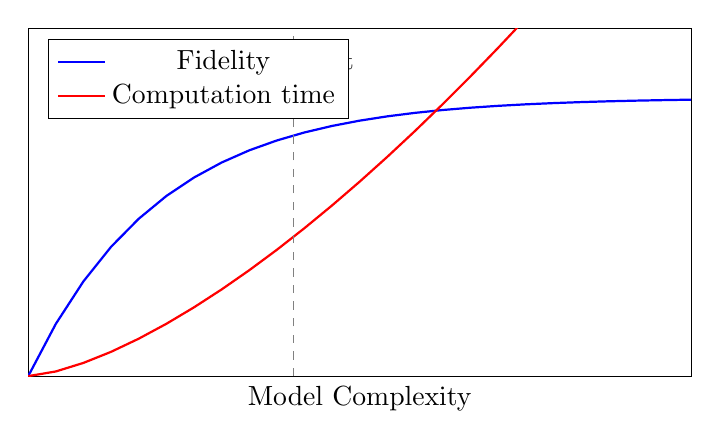
\begin{tikzpicture}
    \begin{axis}[
        width=10cm, height=6cm,
        xlabel={Model Complexity}, ylabel={},
        xmin=0, xmax=10, ymin=0, ymax=10,
        xtick=\empty, ytick=\empty,
        legend pos=north west
    ]
    \addplot[blue, thick, domain=0:10] {8*(1-exp(-0.5*x))};
    \addlegendentry{Fidelity}

    \addplot[red, thick, domain=0:10] {0.5*x^1.5};
    \addlegendentry{Computation time}

    \draw[dashed, gray] (axis cs:4,0) -- (axis cs:4,10);
    \node at (axis cs:4,9) {\small Sweet spot};
    \end{axis}
\end{tikzpicture}
\end{center}

There's a trade-off:
\begin{itemize}
    \item Simple models run fast but may miss important behaviors
    \item Complex models are more accurate but slow (limiting test coverage)
    \item The ``sweet spot'' depends on what behaviors you're testing
\end{itemize}

\section{Validating Simulation Against Hardware}

Before trusting simulation results, validate the model against real hardware:

\begin{enumerate}
    \item \textbf{Static validation}: Compare parameters (mass, inertia, motor constants)
    \item \textbf{Open-loop validation}: Apply same inputs to simulation and hardware, compare outputs
    \item \textbf{Closed-loop validation}: Run same controller on both, compare trajectories
\end{enumerate}

\begin{example}[Validation Procedure]
\begin{enumerate}
    \item Apply a step input to the real quadrotor's attitude controller
    \item Record the attitude response (from motion capture or onboard sensors)
    \item Apply the same step input to the simulation
    \item Compare the responses:
    \begin{itemize}
        \item Rise time should match within 10\%
        \item Overshoot should match within 20\%
        \item Steady-state error should match within 5\%
    \end{itemize}
\end{enumerate}

If discrepancies exist, tune model parameters or add missing dynamics until responses match acceptably.
\end{example}

\section{When to Trust Simulation Results}

\begin{keyidea}[title=Simulation Trust Guidelines]
\begin{itemize}
    \item \textbf{High confidence}: Behaviors that depend on well-modeled dynamics (e.g., controller stability for known parameters)
    \item \textbf{Medium confidence}: Behaviors near operating limits where model accuracy decreases
    \item \textbf{Low confidence}: Behaviors involving unmodeled effects (ground effect, wind turbulence, sensor interference)
\end{itemize}

A test that passes in simulation is \textbf{necessary but not sufficient} for real-world success.
\end{keyidea}

\section{Safety Margins for Uncertainty}

Given model uncertainty, design with margins:

\begin{itemize}
    \item If the spec requires altitude $< 10$ m, design for altitude $< 8$ m in simulation
    \item If the spec allows 30° roll, ensure simulation stays below 25°
    \item General rule: Simulation margin should exceed expected model error
\end{itemize}

\[
\text{Simulation limit} = \text{Spec limit} - \text{Safety margin}
\]
\[
\text{Safety margin} \geq \text{Expected model error}
\]

%======================================================================
\chapter{Multi-Rate Control Systems}
\index{multi-rate control}
%======================================================================

\section{Introduction: The Multi-Rate Problem}

Quadrotor flight controllers are inherently \textbf{multi-rate systems}\index{multi-rate control|textbf}: different control loops run at different frequencies.

\begin{center}
\begin{tabular}{lcc}
\toprule
\textbf{Control Loop} & \textbf{Typical Rate} & \textbf{Rationale} \\
\midrule
Attitude control (inner) & 250--500 Hz & Fast dynamics, stability \\
Rate gyro filtering & 500--2000 Hz & Noise rejection \\
Position control (outer) & 50--100 Hz & Slower dynamics \\
Altitude hold & 50--100 Hz & Barometer/sonar rate \\
Mission planning & 1--10 Hz & High-level decisions \\
\bottomrule
\end{tabular}
\end{center}

\textbf{Why different rates?}

\begin{itemize}
    \item \textbf{Dynamics timescales}: Attitude dynamics are fast (time constant ~50 ms); position dynamics are slow (time constant ~1 s). Control theory dictates that sampling rate should be 10--20$\times$ faster than the closed-loop bandwidth.

    \item \textbf{Sensor rates}: IMU can output at 1 kHz+; GPS outputs at 5--10 Hz. Control loops must match sensor availability.

    \item \textbf{Computational cost}: Higher rates require more CPU. Running all loops at the fastest rate wastes resources.
\end{itemize}

\section{Cascaded Control Architecture}

The standard quadrotor control architecture is \textbf{cascaded}: outer loops generate setpoints for inner loops.

\begin{center}
\begin{tikzpicture}[node distance=1.5cm, >=Stealth]
    \node[draw, rectangle, minimum width=2.5cm, minimum height=1cm] (pos) {Position Controller (50 Hz)};
    \node[draw, rectangle, minimum width=2.5cm, minimum height=1cm, right=of pos] (att) {Attitude Controller (500 Hz)};
    \node[right=of att] (motor) {Motors};
    \node[left=of pos] (cmd) {Position Cmd};

    \draw[->] (cmd) -- (pos);
    \draw[->] (pos) -- node[above] {Attitude Setpoint} (att);
    \draw[->] (att) -- node[above] {Motor Cmd} (motor);
\end{tikzpicture}
\end{center}

\textbf{Why cascade?}
\begin{enumerate}
    \item \textbf{Timescale separation}: Inner loops are much faster than outer loops, allowing them to be designed independently.
    \item \textbf{Physical structure}: Position changes through attitude (you tilt to move), so attitude control is a natural inner loop.
    \item \textbf{Tuning simplicity}: Tune inner loop first (assuming outer loop is constant), then tune outer loop (assuming inner loop is ideal).
\end{enumerate}

\begin{keyidea}[title=Timescale Separation Principle]
For cascaded control to work well, the inner loop must be significantly faster than the outer loop (typically 5--10$\times$). This allows the outer loop to ``see'' the inner loop as nearly instantaneous.

For quadrotors:
\begin{itemize}
    \item Attitude bandwidth: 10--20 rad/s
    \item Position bandwidth: 1--2 rad/s
    \item Ratio: ~10$\times$ \checkmark
\end{itemize}
\end{keyidea}

\section{Multi-Rate Task Design}

\subsection{Rate Relationships}

The cleanest multi-rate designs use \textbf{harmonic rates}: each slow rate is an integer divisor of faster rates.

\begin{example}[Harmonic Rate Design]
Base rate: 1 ms (1000 Hz)
\begin{itemize}
    \item IMU sampling: every 1 ms (1000 Hz)
    \item Attitude control: every 2 ms (500 Hz)
    \item Position control: every 20 ms (50 Hz)
    \item Telemetry: every 100 ms (10 Hz)
\end{itemize}

All rates are integer multiples of the base rate, ensuring consistent timing relationships.
\end{example}

\subsection{Rate Transitions}

When data flows between tasks running at different rates, we need \textbf{rate transition} handling:

\textbf{Fast-to-Slow (Downsampling)}:
The slow task reads data produced by the fast task. Options:
\begin{itemize}
    \item \textbf{Latest value}: Use the most recent value (simple, but aliases fast changes)
    \item \textbf{Averaging}: Average values over the slow period (filters noise)
\end{itemize}

\textbf{Slow-to-Fast (Upsampling)}:
The fast task uses data produced by the slow task. Options:
\begin{itemize}
    \item \textbf{Hold}: Use the same value until the slow task updates (creates steps)
    \item \textbf{Interpolation}: Linearly interpolate between slow updates (smoother but adds delay)
\end{itemize}

\subsection{Data Consistency}

\begin{warningbox}[title=Multi-Rate Data Consistency]
When slow and fast tasks share data, ensure consistency:
\begin{enumerate}
    \item The slow task should update all related variables atomically
    \item The fast task should copy all related variables atomically
    \item Never read some variables, release lock, then read more related variables
\end{enumerate}
\end{warningbox}

\section{Timing Analysis for Multi-Rate Systems}

Consider a system with three rates:

\begin{itemize}
    \item Task A: Period 2 ms, WCET 0.5 ms (attitude control)
    \item Task B: Period 10 ms, WCET 2 ms (position control)
    \item Task C: Period 20 ms, WCET 3 ms (state estimation)
\end{itemize}

At $t = 0$, all tasks are released simultaneously (the \textbf{critical instant}). With RMS priorities:

\begin{enumerate}
    \item Task A (highest priority) runs first: completes at 0.5 ms
    \item Task A releases again at 2 ms, preempts whatever is running
    \item Task B runs when A is not ready
    \item Task C (lowest priority) runs in remaining gaps
\end{enumerate}

The critical instant produces the worst-case response times used in schedulability analysis.

\section{Design Guidelines}

\begin{keyidea}[title=Multi-Rate Design Guidelines]
\begin{enumerate}
    \item Use \textbf{harmonic rates} (integer multiples) for predictable timing
    \item Ensure \textbf{timescale separation} (5--10$\times$) between cascaded loops
    \item Handle \textbf{rate transitions} explicitly (hold, interpolate, or average)
    \item Verify \textbf{schedulability} considering all rates
    \item Test at the \textbf{critical instant} when all tasks release simultaneously
\end{enumerate}
\end{keyidea}
